\documentclass[
]{jss}

%% recommended packages
\usepackage{orcidlink,thumbpdf,lmodern}

\usepackage[utf8]{inputenc}

\author{
H. Sherry Zhang\\Monash University \And Dianne Cook\\Monash University \AND Ursula Laa\\University of Natural Resources and Life Sciences \AND Nicolas Langrené\\BNU-HKBU United International College \AND Patricia Menéndez\\Monash University \AND
}
\title{\pkg{cubble}: An R Package for Structuring Spatio-temporal Data}

\Plainauthor{H. Sherry Zhang, Dianne Cook, Ursula Laa, Nicolas Langrené, Patricia Menéndez}
\Plaintitle{cubble: An R Package for Structuring Spatio-temporal Data}


\Abstract{
Spatio-temporal data refer to measurements taken across space and time. In practice, spatio-temporal data can be decomposed into a spatial and temporal component: at one time, we would select a spatial location and inspect the temporal trend; at other time, we might select one or multiple time value(s) and explore the spatial distribution. Ideally, we could make multiple maps and multiple time series to explore these together, however, doing all of these actions is complicated when data arrive fragmented in multiple objects. To make it easy to do all these tasks, ideally spatial and temporal variables are in a single data object that we can slice and dice in different ways to conduct different visualisations. This work suggests a new data structure, \code{cubble}, that uses a nested form and a long form to organise spatial and temporal variables in a single data object. The new data structure ensures that data in the two forms are synchronised while been flexible to explore the two aspect of spatio-temporal data. It also provides capability for handling data with hierarchical structure, matching data from multiple sources, constructing interactive graphics, and performing spatio-temporal transformation. The paper will demonstrate \pkg{cubble} with examples using Australian climate weather stations, river level data, and climate reanalysis (ERA5) data.
}

\Keywords{spatial, temporal, spatio temporal, \proglang{R}, environmental data, exploratory data analysis}
\Plainkeywords{spatial, temporal, spatio temporal, R, environmental data, exploratory data analysis}

%% publication information
%% \Volume{50}
%% \Issue{9}
%% \Month{June}
%% \Year{2012}
%% \Submitdate{}
%% \Acceptdate{2012-06-04}

\Address{
    H. Sherry Zhang\\
    Monash University\\
    21 Chancellors Walk, Clayton VIC 3800 Australia\\
  E-mail: \email{huize.zhang@monash.edu}\\
  
      Dianne Cook\\
    Monash University\\
    21 Chancellors Walk, Clayton VIC 3800 Australia\\
  E-mail: \href{mailto:dicook@monash.edu}{\nolinkurl{dicook@monash.edu}}\\
  
      Ursula Laa\\
    University of Natural Resources and Life Sciences\\
    Gregor-Mendel-Straße 33, 1180 Wien, Austria\\
  E-mail: \href{mailto:ursula.laa@boku.ac.at}{\nolinkurl{ursula.laa@boku.ac.at}}\\
  
      Nicolas Langrené\\
    BNU-HKBU United International College\\
    2000 Jintong Road, Tangjiawan, Zhuhai, Guangdong Province, China\\
  E-mail: \href{mailto:nicolaslangrene@uic.edu.cn}{\nolinkurl{nicolaslangrene@uic.edu.cn}}\\
  
      Patricia Menéndez\\
    Monash University\\
    21 Chancellors Walk, Clayton VIC 3800 Australia\\
  E-mail: \href{mailto:patricia.menendez@monash.edu}{\nolinkurl{patricia.menendez@monash.edu}}\\
  
  }

% Pandoc syntax highlighting
\usepackage{color}
\usepackage{fancyvrb}
\newcommand{\VerbBar}{|}
\newcommand{\VERB}{\Verb[commandchars=\\\{\}]}
\DefineVerbatimEnvironment{Highlighting}{Verbatim}{commandchars=\\\{\}}
% Add ',fontsize=\small' for more characters per line
\usepackage{framed}
\definecolor{shadecolor}{RGB}{248,248,248}
\newenvironment{Shaded}{\begin{snugshade}}{\end{snugshade}}
\newcommand{\AlertTok}[1]{\textcolor[rgb]{0.94,0.16,0.16}{#1}}
\newcommand{\AnnotationTok}[1]{\textcolor[rgb]{0.56,0.35,0.01}{\textbf{\textit{#1}}}}
\newcommand{\AttributeTok}[1]{\textcolor[rgb]{0.77,0.63,0.00}{#1}}
\newcommand{\BaseNTok}[1]{\textcolor[rgb]{0.00,0.00,0.81}{#1}}
\newcommand{\BuiltInTok}[1]{#1}
\newcommand{\CharTok}[1]{\textcolor[rgb]{0.31,0.60,0.02}{#1}}
\newcommand{\CommentTok}[1]{\textcolor[rgb]{0.56,0.35,0.01}{\textit{#1}}}
\newcommand{\CommentVarTok}[1]{\textcolor[rgb]{0.56,0.35,0.01}{\textbf{\textit{#1}}}}
\newcommand{\ConstantTok}[1]{\textcolor[rgb]{0.00,0.00,0.00}{#1}}
\newcommand{\ControlFlowTok}[1]{\textcolor[rgb]{0.13,0.29,0.53}{\textbf{#1}}}
\newcommand{\DataTypeTok}[1]{\textcolor[rgb]{0.13,0.29,0.53}{#1}}
\newcommand{\DecValTok}[1]{\textcolor[rgb]{0.00,0.00,0.81}{#1}}
\newcommand{\DocumentationTok}[1]{\textcolor[rgb]{0.56,0.35,0.01}{\textbf{\textit{#1}}}}
\newcommand{\ErrorTok}[1]{\textcolor[rgb]{0.64,0.00,0.00}{\textbf{#1}}}
\newcommand{\ExtensionTok}[1]{#1}
\newcommand{\FloatTok}[1]{\textcolor[rgb]{0.00,0.00,0.81}{#1}}
\newcommand{\FunctionTok}[1]{\textcolor[rgb]{0.00,0.00,0.00}{#1}}
\newcommand{\ImportTok}[1]{#1}
\newcommand{\InformationTok}[1]{\textcolor[rgb]{0.56,0.35,0.01}{\textbf{\textit{#1}}}}
\newcommand{\KeywordTok}[1]{\textcolor[rgb]{0.13,0.29,0.53}{\textbf{#1}}}
\newcommand{\NormalTok}[1]{#1}
\newcommand{\OperatorTok}[1]{\textcolor[rgb]{0.81,0.36,0.00}{\textbf{#1}}}
\newcommand{\OtherTok}[1]{\textcolor[rgb]{0.56,0.35,0.01}{#1}}
\newcommand{\PreprocessorTok}[1]{\textcolor[rgb]{0.56,0.35,0.01}{\textit{#1}}}
\newcommand{\RegionMarkerTok}[1]{#1}
\newcommand{\SpecialCharTok}[1]{\textcolor[rgb]{0.00,0.00,0.00}{#1}}
\newcommand{\SpecialStringTok}[1]{\textcolor[rgb]{0.31,0.60,0.02}{#1}}
\newcommand{\StringTok}[1]{\textcolor[rgb]{0.31,0.60,0.02}{#1}}
\newcommand{\VariableTok}[1]{\textcolor[rgb]{0.00,0.00,0.00}{#1}}
\newcommand{\VerbatimStringTok}[1]{\textcolor[rgb]{0.31,0.60,0.02}{#1}}
\newcommand{\WarningTok}[1]{\textcolor[rgb]{0.56,0.35,0.01}{\textbf{\textit{#1}}}}

% tightlist command for lists without linebreak
\providecommand{\tightlist}{%
  \setlength{\itemsep}{0pt}\setlength{\parskip}{0pt}}

% From pandoc table feature
\usepackage{longtable,booktabs,array}
\usepackage{calc} % for calculating minipage widths
% Correct order of tables after \paragraph or \subparagraph
\usepackage{etoolbox}
\makeatletter
\patchcmd\longtable{\par}{\if@noskipsec\mbox{}\fi\par}{}{}
\makeatother
% Allow footnotes in longtable head/foot
\IfFileExists{footnotehyper.sty}{\usepackage{footnotehyper}}{\usepackage{footnote}}
\makesavenoteenv{longtable}



\usepackage{amsmath} \usepackage{array} \usepackage{xcolor} \newcommand{\sherry}[1]{\textcolor{magenta}{#1}}

\begin{document}



\newpage

\hypertarget{introduction}{%
\section{Introduction}\label{introduction}}

Spatio-temporal data has a spatial component referring to the location of each observation, a temporal component that is recorded at regular or irregular time intervals, and may have multiple variables measured at each spatial and temporal value. The analysis of spatio-temporal data can fix the time to explore the spatial distribution, fix the spatial location to explore temporal trends, or dynamically explore the space and time simultaneously. For these tasks to be carried out easily, there is a need for a spatio-temporal data representation that underpins various operations.

The \emph{Representing data} section of the SpatioTemproal CRAN task view \citep{ctvspatiotemporal} lists existing spatio-temporal data representation. Among them, \citet{spacetime} proposes four layouts: full grid layout, sparse grid layout, irregular layout, and trajectory. These layouts are implemented in the \pkg{spacetime} \citep{spacetime} package with the underlying spatial and temporal class: \pkg{sp} \citep{sp} and \pkg{xts} \citep{xts}. The \pkg{stars} \citep{stars} package has been a recent implementation to handle both raster and vector spatio-temporal data using array. It depends on the newer spatial package \pkg{sf} \citep{sf} and interfaces with the widely-used tidyverse verbs.

{[}till here{]} One issue with wrangling spatio-temporal data is that the raw data does not naturally structured in any one of the representation above. Also, in data collection, spatio-temporal data is less often collected as a whole piece but fragmented spatial and temporal data for analysts to ensemble. For example, map data records the shape of a collection of area of interest is provided by official government website; geo-scientific data records the longitude and latitude coordinate of locations in the area along with other meta data relates to the location; and temporal variables indexed by both location and time. For spatio-temporal data analysis, merging all these sources can be challenging and joining these tables can go wrong because of the slightest unmatched of the linking variable from different sources.

Another issue is how the concept of tidy data \citep{tidydata} should be applied to spatio-temporal data. The tidy data concept advocates the data to be shaped into 1) one row per observation; 2) one column per variable; and 3) one type of data per table. The long form data is preferred over wide data given the downstream software i.e.~\pkg{dplyr} and \pkg{ggplot2} for data wrangling and visualisation. However, the long form can be inefficient to store feature geometries, especially for large multipolygon over long time period. This poses the question on how to arrange spatial and temporal variables that makes analysing spatio-temporal data easier.

This paper presents a new \proglang{R} package, \pkg{cubble}, to {[}overcome the problem{]} with organising variables in different levels when working with spatio-temporal data. The data structure focuses on connecting to the upstream data collection and is suitable for temporal data collected at the fixed location over time. Among the four spacetime layouts in \citet{spacetime}, it can be full grid layout, sparse grid layout, or irregular layout, but trajectory is not within the scope of this work. In the package a new data structure, also called \code{cubble}, is proposed to organise spatial and temporal variables as two forms of a single data object so that they can be wrangled separately while synchronised as a whole piece. With this new data object, analysts can spend less time writing codes to organise spatial and temporal variables and focus more on the exploratory data analysis itself. The software is available from the Comprehensive R Archive Network (CRAN) at {[}CRAN link{]}.

The rest of the paper is divided as follows: Section \ref{cube} discusses the spatio-temporal cube to conceptualise spatio-temporal data. Section \ref{cubble} presents the main design and functionality of \pkg{cubble}. Section \ref{others} explains how cubble deals with more advanced considerations including data with hierarchical structure, data matching, how cubble fits with existing static and interactive visualisation tools, and spatio-temporal data transformation. Section \ref{examples} uses Australia weather station data and river level data as examples to demonstrate the use of \pkg{cubble}. An example on how \pkg{cubble} handles NetCDF data is also provided. Section \ref{conclude} concludes the paper.

\hypertarget{cube}{%
\section{Conceptual framework: spatio-temporal cube}\label{cube}}

Spatio-temporal data can be conceptualised using a cubical data model with reference to variables, time and space. This naturally motivates the usage of array to represent and store spatio-temporal data, as evident by satellite imageries, large climate models, among others. The work by \citet{lu_multidimensional_2018} has discussed the suitability of this representation through array algebra and practical spatio-temporal tasks. \textcolor{magenta}{SZ: is this too direct?}

The cubical conceptual framework provides a generalisation to the operation can be done on the data for visualisation. A paper by \citet{bach_review_2014} has reviewed the temporal data visualisation based on space-time cube operations. Notice that the term space-time cube in their article ``does not need to involve spatial data'', but referring to ``an abstract 2D substrate that is used to visualize data at a specific time''. Despite its main focus is on temporal data, the mindset of abstracting out data representation to construct visualisation is applicable to our spatio-temporal data manipulation and visualisation.

\hypertarget{cubble}{%
\section{The cubble package}\label{cubble}}

This section will first introduce the core functions in the cubble class: \code{as_cubble()}, \code{face_spatial()}, \code{face_temporal()}, and \code{unfold()} from subsection \ref{create} to \ref{unfold}. The next subsection addresses why bother a new class before subsection \ref{compact} finishing on the compatibility of cubble with existing packages in spatial and temporal analysis.

Each core function is introduced with a short example accompanied and the data \texttt{climate\_flat} is used throughout this section. \texttt{climate\_flat} contains five weather stations in Australia with spatial information of each station: station id, latitude, longitude, elevation, station name and World Meteorology Organisation ID and also daily temporal information of date, maximum and minimum temperature and precipitation for 2020. Below prints out the first five rows of \texttt{climate\_flat}:

\begin{CodeChunk}
\begin{CodeOutput}
# A tibble: 1,830 x 10
  id            lat  long  elev name         wmo_id date        prcp  tmax  tmin
  <chr>       <dbl> <dbl> <dbl> <chr>         <dbl> <date>     <dbl> <dbl> <dbl>
1 ASN00009021 -31.9  116.  15.4 perth airpo~  94610 2020-01-01     0  31.9  15.3
2 ASN00009021 -31.9  116.  15.4 perth airpo~  94610 2020-01-02     0  24.9  16.4
3 ASN00009021 -31.9  116.  15.4 perth airpo~  94610 2020-01-03     6  23.2  13  
4 ASN00009021 -31.9  116.  15.4 perth airpo~  94610 2020-01-04     0  28.4  12.4
5 ASN00009021 -31.9  116.  15.4 perth airpo~  94610 2020-01-05     0  35.3  11.6
# ... with 1,825 more rows
\end{CodeOutput}
\end{CodeChunk}

\hypertarget{create}{%
\subsection{Create a cubble in the nested form}\label{create}}

As described in the introduction, spatio-temporal data can come in various formats and shapes. A cubble can be created from various raw data, including tibble and its variates multiple tables (an example provided in section \ref{covid}), and netcdf (detailed in section \ref{netcdf}). The function \code{as_cubble()} is used to create a cubble with three additional components: \code{key} as the spatial identifier; \code{index} as the temporal identifier; and a vector of \code{coords} in the order of longitude and latitude. Argument \code{key} and \code{index} follow the wording in \pkg{tsibble} to define temporal order and multiple series while \code{coords} is a space specific argument to locate each site in two columns. The code below creates a cubble out of \code{climate_flat} with \code{id} as the key, \code{date} as the index, and \code{c(long, lat)} as the coordinates:

\begin{CodeChunk}
\begin{CodeInput}
R> cubble_nested <- climate_flat |>
+   as_cubble(key = id, index = date, coords = c(long, lat))
R> cubble_nested
\end{CodeInput}
\begin{CodeOutput}
# cubble:   id [5]: nested form
# bbox:     [115.97, -32.94, 133.55, -12.42]
# temporal: date [date], prcp [dbl], tmax [dbl], tmin [dbl]
  id            lat  long  elev name           wmo_id ts                
  <chr>       <dbl> <dbl> <dbl> <chr>           <dbl> <list>            
1 ASN00009021 -31.9  116.  15.4 perth airport   94610 <tibble [366 x 4]>
2 ASN00010311 -31.9  117. 179   york            94623 <tibble [366 x 4]>
3 ASN00010614 -32.9  117. 338   narrogin        94627 <tibble [366 x 4]>
4 ASN00014015 -12.4  131.  30.4 darwin airport  94120 <tibble [366 x 4]>
5 ASN00015131 -17.6  134. 220   elliott         94236 <tibble [366 x 4]>
\end{CodeOutput}
\end{CodeChunk}

The cubble header provides some information about this data. \code{id} is the variable name to identify each location and there are five unique locations. The bounding box is \code{[115.97, -32.94, 133.55, -12.42]} and the names of variable nested in the \code{ts} column, along with its type, are \code{date [date], prcp [dbl], tmax [dbl], tmin [dbl]}.

The created cubble is built from a \code{rowwise_df} class where each row forms a group and all the temporal variables are nested in a list column, hence it is also called the nested cubble. The rowwise structure makes it simpler to calculate on the list using \code{mutate()} and avoid the \code{map()} when working with list column. For example calculating the number of raining day can be done by:

\begin{CodeChunk}
\begin{CodeOutput}
# cubble:   id [5]: nested form
# bbox:     [115.97, -32.94, 133.55, -12.42]
# temporal: date [date], prcp [dbl], tmax [dbl], tmin [dbl]
  id            lat  long  elev name           wmo_id ts       rain_day
  <chr>       <dbl> <dbl> <dbl> <chr>           <dbl> <list>      <int>
1 ASN00009021 -31.9  116.  15.4 perth airport   94610 <tibble>      104
2 ASN00010311 -31.9  117. 179   york            94623 <tibble>       89
3 ASN00010614 -32.9  117. 338   narrogin        94627 <tibble>       90
4 ASN00014015 -12.4  131.  30.4 darwin airport  94120 <tibble>      106
5 ASN00015131 -17.6  134. 220   elliott         94236 <tibble>       63
\end{CodeOutput}
\end{CodeChunk}

\hypertarget{switch-from-the-nested-cubble-into-the-long-form}{%
\subsection{Switch from the nested cubble into the long form}\label{switch-from-the-nested-cubble-into-the-long-form}}

The nested format is convenient for those operations whose output does not contain a time dimension. For those outputs that are cross-identified by the spatial and temporal identifier, a long cubble needs to be used. The function \code{face_temporal()} switches the cubble from the nested form to the long form and the first row in Figure \ref{fig:face} sketches the function in a diagram. This code shows how to switch the cubble just created into its long form:

\begin{CodeChunk}
\begin{CodeInput}
R> cubble_long <- cubble_nested |> face_temporal()
R> cubble_long
\end{CodeInput}
\begin{CodeOutput}
# cubble:  date, id [5]: long form
# bbox:    [115.97, -32.94, 133.55, -12.42]
# spatial: lat [dbl], long [dbl], elev [dbl], name [chr], wmo_id [dbl]
  id          date        prcp  tmax  tmin
  <chr>       <date>     <dbl> <dbl> <dbl>
1 ASN00009021 2020-01-01     0  31.9  15.3
2 ASN00009021 2020-01-02     0  24.9  16.4
3 ASN00009021 2020-01-03     6  23.2  13  
4 ASN00009021 2020-01-04     0  28.4  12.4
5 ASN00009021 2020-01-05     0  35.3  11.6
# ... with 1,825 more rows
\end{CodeOutput}
\end{CodeChunk}

Notice that the third line in the header now shows the name and type of spatial variables: \code{lat [dbl], long [dbl], elev [dbl], name [chr], wmo_id [dbl]} and these variables are now stored as a \code{spatial} attribute of the data:

\begin{CodeChunk}
\begin{CodeInput}
R> attr(cubble_long, "spatial")
\end{CodeInput}
\begin{CodeOutput}
# A tibble: 5 x 6
  id            lat  long  elev name           wmo_id
  <chr>       <dbl> <dbl> <dbl> <chr>           <dbl>
1 ASN00009021 -31.9  116.  15.4 perth airport   94610
2 ASN00010311 -31.9  117. 179   york            94623
3 ASN00010614 -32.9  117. 338   narrogin        94627
4 ASN00014015 -12.4  131.  30.4 darwin airport  94120
5 ASN00015131 -17.6  134. 220   elliott         94236
\end{CodeOutput}
\end{CodeChunk}

The long form is built form class \code{groupped_df} where all the observations from the same sites forms a group.

\begin{CodeChunk}
\begin{figure}

{\centering 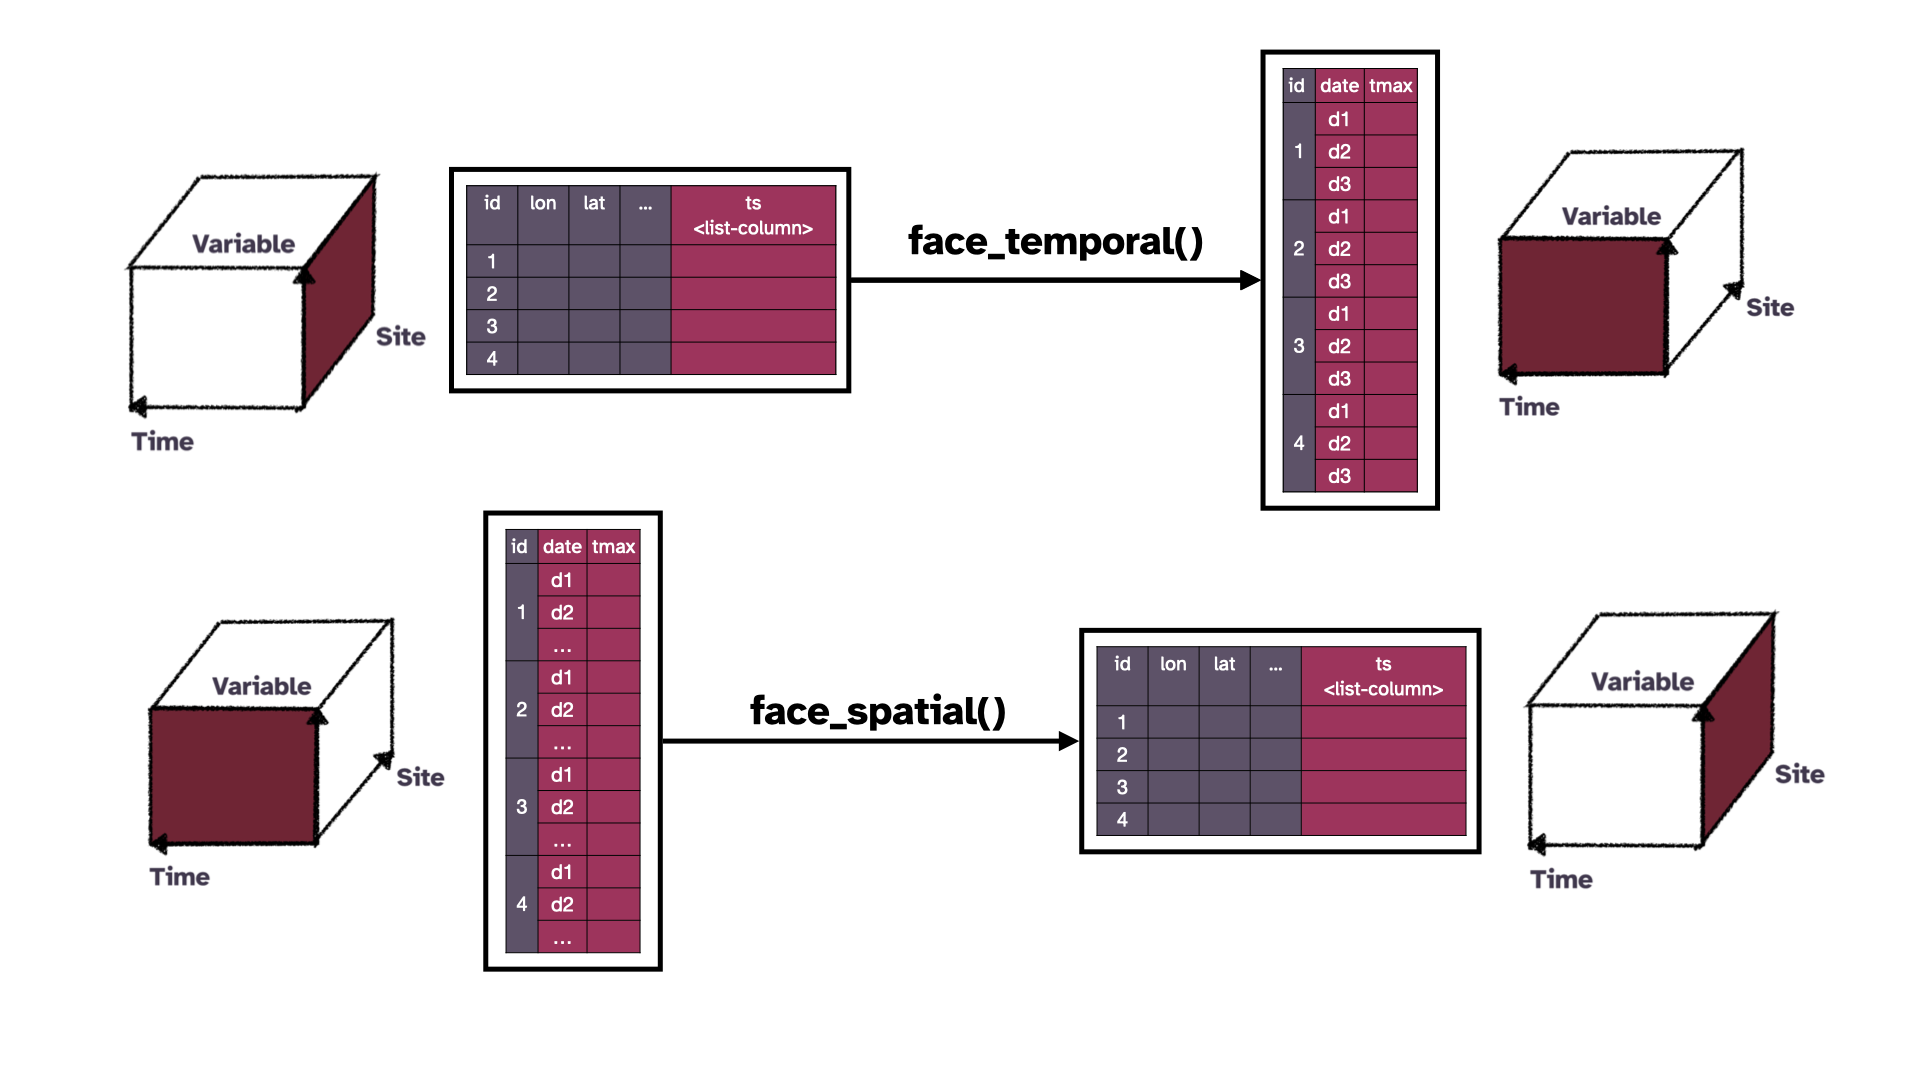
\includegraphics[width=1\linewidth]{/Users/sherryzhang/Documents/research/paper-cubble/figures/diagram-keynotes/diagram-keynotes.008} 

}

\caption{An illustration of function \code{face\_temporal} and \code{face\_spatial} in cubble. In the first row, \code{face\_temporal} switches a cubble from the nested form into the long form and the focus has switched from the spatial aspect (the side face) to the temporal aspect (the front face). In the second row, \code{face\_spatial} switches a cubble back to the nested form from te long form and shift focus back to the spatial aspect.}\label{fig:face}
\end{figure}
\end{CodeChunk}

\hypertarget{switch-a-long-cubble-back-to-the-nested-form}{%
\subsection{Switch a long cubble back to the nested form}\label{switch-a-long-cubble-back-to-the-nested-form}}

Manipulation on the spatial and temporal dimension can be an iterative process and analysts may need to go back and forth between the nested and long cubble. \code{face_spatial()}, the inverse of \code{face_temporal()}, switches the long cubble back to the nested form, as sketched in the second row in Figure \ref{fig:face}:

\begin{CodeChunk}
\begin{CodeInput}
R> cubble_back <- cubble_long |> face_spatial()
R> cubble_back
\end{CodeInput}
\begin{CodeOutput}
# cubble:   id [5]: nested form
# bbox:     [115.97, -32.94, 133.55, -12.42]
# temporal: date [date], prcp [dbl], tmax [dbl], tmin [dbl]
  id            lat  long  elev name           wmo_id ts                
  <chr>       <dbl> <dbl> <dbl> <chr>           <dbl> <list>            
1 ASN00009021 -31.9  116.  15.4 perth airport   94610 <tibble [366 x 4]>
2 ASN00010311 -31.9  117. 179   york            94623 <tibble [366 x 4]>
3 ASN00010614 -32.9  117. 338   narrogin        94627 <tibble [366 x 4]>
4 ASN00014015 -12.4  131.  30.4 darwin airport  94120 <tibble [366 x 4]>
5 ASN00015131 -17.6  134. 220   elliott         94236 <tibble [366 x 4]>
\end{CodeOutput}
\end{CodeChunk}

\hypertarget{unfold}{%
\subsection{Flatten spatial variables into the long cubble}\label{unfold}}

Sometimes, analysts may need to apply some variable transformation that involves both the spatial and temporal variable. An example of this is the transformation of temporal variables into the spatial dimension in glyph maps, which will be elaborated in section \ref{st_transformation}. This type of operations can be seen as flattening, or \emph{unfolding}, the cube into a 2D data frame. Here the function \code{unfold()} moves the spatial variables \code{long} and \code{lat} into the long cubble:

\begin{CodeChunk}
\begin{CodeInput}
R> cubble_unfold <- cubble_long |> unfold(long, lat)
R> cubble_unfold
\end{CodeInput}
\begin{CodeOutput}
# cubble:  date, id [5]: long form
# bbox:    [115.97, -32.94, 133.55, -12.42]
# spatial: lat [dbl], long [dbl], elev [dbl], name [chr], wmo_id [dbl]
  id          date        prcp  tmax  tmin  long   lat
  <chr>       <date>     <dbl> <dbl> <dbl> <dbl> <dbl>
1 ASN00009021 2020-01-01     0  31.9  15.3  116. -31.9
2 ASN00009021 2020-01-02     0  24.9  16.4  116. -31.9
3 ASN00009021 2020-01-03     6  23.2  13    116. -31.9
4 ASN00009021 2020-01-04     0  28.4  12.4  116. -31.9
5 ASN00009021 2020-01-05     0  35.3  11.6  116. -31.9
# ... with 1,825 more rows
\end{CodeOutput}
\end{CodeChunk}

This function should generally be used in the last step of the analysis since it is a temporary operation, meaning these added spatial variables are not stored in the long form and will disappear if switched to the nested form and then switched back:

\begin{CodeChunk}
\begin{CodeInput}
R> cubble_unfold |> face_spatial() |> face_temporal()
\end{CodeInput}
\begin{CodeOutput}
# cubble:  date, id [5]: long form
# bbox:    [115.97, -32.94, 133.55, -12.42]
# spatial: lat [dbl], long [dbl], elev [dbl], name [chr], wmo_id [dbl]
  id          date        prcp  tmax  tmin
  <chr>       <date>     <dbl> <dbl> <dbl>
1 ASN00009021 2020-01-01     0  31.9  15.3
2 ASN00009021 2020-01-02     0  24.9  16.4
3 ASN00009021 2020-01-03     6  23.2  13  
4 ASN00009021 2020-01-04     0  28.4  12.4
5 ASN00009021 2020-01-05     0  35.3  11.6
# ... with 1,825 more rows
\end{CodeOutput}
\end{CodeChunk}

\subsection[Why not just use]{Why not just use \code{dplyr::nest\_by()}}

It may naturally raise the question that why bother a new data structure since the nested form can already be created by the \pkg{dplyr} function \code{nest_by()}? While \code{nest_by()} and \code{unnest()} can mimic the nested form in cubble, cubble can be seen as an attempt to arrange variables from different observational units into a single object, specifically for spatio-temporal data. While \texttt{nest\_by()} solves this problem on the spatial side, it doesn't solve the temporal side. For temporal data, a combined representation with spatial variables is useful for spatio-temporal operations but its duplication can be a burden to operate on. Also, spatial variables are dropped when summarised and you will need to either specified all of them in the \code{group_by()} before \code{summarise}, or add a joining after \code{summarise()}.

\hypertarget{compact}{%
\subsection{Compatibility with existing packages}\label{compact}}

The previous four subsections have introduced operations specific to the \code{cubble} class and this section will demonstrate how the \code{cubble} class interacts with existing packages commonly used in spatial and temporal analysis, specifically, \code{dplyr}, \code{tsibble}, \code{sf} (\code{s2}), and \code{netcdf4}.

\hypertarget{dplyr}{%
\subsubsection{dplyr}\label{dplyr}}

The \code{dplyr} package has provided many tools for data wrangling tasks and these operations are useful in the spatio-temporal context. \code{cubble} provides methods that support the following \code{dplyr} verbs in both the nested and long form:

\begin{quote}
\texttt{mutate}, \texttt{filter}, \texttt{summarise}, \texttt{select}, \texttt{arrange}, \texttt{rename}, \texttt{left\_join}, and the slice family (\texttt{slice\_head}, \texttt{slice\_tail}, \texttt{slice\_sample}, \texttt{slice\_min}, \texttt{slice\_max})
\end{quote}

\hypertarget{tsibble}{%
\subsubsection{tsibble}\label{tsibble}}

\code{tsibble} is a temporal data structure that uses \code{index} and \code{key} to identify the time and different series. \code{cubble} can be seen as following the same vein as \code{tsibble} for spatio-temporal data. This makes it easy to cast a \code{tsibble} into a \code{cubble} as only the \code{coords} argument needs to be supplied:

\begin{CodeChunk}
\begin{CodeInput}
R> # example with a tsibble created from climate_flat
R> raw <- climate_flat |> tsibble::as_tsibble(key = id, index = date)
R> dt <-  raw |> cubble::as_cubble(coords = c(long, lat))
R> dt
\end{CodeInput}
\begin{CodeOutput}
# cubble:   id [5]: nested form
# bbox:     [115.97, -32.94, 133.55, -12.42]
# temporal: date [date], prcp [dbl], tmax [dbl], tmin [dbl]
  id            lat  long  elev name           wmo_id ts                
  <chr>       <dbl> <dbl> <dbl> <chr>           <dbl> <list>            
1 ASN00009021 -31.9  116.  15.4 perth airport   94610 <tbl_ts [366 x 4]>
2 ASN00010311 -31.9  117. 179   york            94623 <tbl_ts [366 x 4]>
3 ASN00010614 -32.9  117. 338   narrogin        94627 <tbl_ts [366 x 4]>
4 ASN00014015 -12.4  131.  30.4 darwin airport  94120 <tbl_ts [366 x 4]>
5 ASN00015131 -17.6  134. 220   elliott         94236 <tbl_ts [366 x 4]>
\end{CodeOutput}
\end{CodeChunk}

In the nested cubble created, each element in the list-column \code{ts} is of \code{tbl_ts} class and operations available to the tsibble class is still valid under cubble. For example, the code below calculates two features of the maximum temperature:

\begin{CodeChunk}
\begin{CodeInput}
R> # add station-based features in the nested form.
R> dt |> mutate(fabletools::features(ts, tmax, list(tmax_mean = mean, tmax_var = var)))
\end{CodeInput}
\begin{CodeOutput}
# cubble:   id [5]: nested form
# bbox:     [115.97, -32.94, 133.55, -12.42]
# temporal: date [date], prcp [dbl], tmax [dbl], tmin [dbl]
  id            lat  long  elev name          wmo_id ts       tmax_mean tmax_var
  <chr>       <dbl> <dbl> <dbl> <chr>          <dbl> <list>       <dbl>    <dbl>
1 ASN00009021 -31.9  116.  15.4 perth airport  94610 <tbl_ts>      25.7    38.6 
2 ASN00010311 -31.9  117. 179   york           94623 <tbl_ts>      26.2    51.1 
3 ASN00010614 -32.9  117. 338   narrogin       94627 <tbl_ts>      23.7    45.4 
4 ASN00014015 -12.4  131.  30.4 darwin airpo~  94120 <tbl_ts>      33.1     3.02
5 ASN00015131 -17.6  134. 220   elliott        94236 <tbl_ts>      34.6    24.7 
\end{CodeOutput}
\end{CodeChunk}

\hypertarget{sf-and-s2}{%
\subsubsection{sf and s2}\label{sf-and-s2}}

As a spatial data object, \code{sf} creates a simple feature geometry list-column (\code{sfc}) in the data frame to provide spatial operations on various geometry types (\code{POINT}, \code{LINESTRING}, \code{POLYGON}, \code{MULTIPOLYGON}, etc). These spatial operations are also valuable for spatio-temporal data analysis, but an \code{sf} object \emph{usually} does not contain temporal variables. This means \code{sf} cannot be directly cast into a \code{cubble}, however, \code{cubble} does support \code{sfc} columns in the nested form and spatial operations applied to the \code{sfc} column in \code{sf} can still be applied to the \code{sfc} column in a cubble. The following example shows how to create an \code{sfc} column of \code{POINT} type from latitude and longitude in cubble. Then \code{sf::st_within} is used to add the state \code{MULTIPOLYGON} of each weather station before a coordinate transformation is made.

\begin{CodeChunk}
\begin{CodeInput}
R> library(sf)
R> # create a cubble
R> cb <- climate_flat |>
+   cubble::as_cubble(key = id, index = date, coords = c(long, lat))
R> 
R> aus <- ozmaps::abs_ste
R> 
R> dt <- cb |>
+   mutate(
+     # create `sfc` column based on long and lat
+     ll = st_sfc(
+       purrr::map2(long, lat, ~st_point(c(.x, .y))),
+       crs = st_crs(aus)),
+ 
+     # append state multi-polygon based on the `sfc` created
+     state = aus$geometry[st_within(ll, aus, sparse = FALSE)],
+ 
+     # adopt a different projection: lambert conformal conic (EPSG:3112)
+     state = st_transform(state, crs = "EPSG:3112")
+     )
R> 
R> dt
\end{CodeInput}
\begin{CodeOutput}
# cubble:   id [5]: nested form
# bbox:     [115.97, -32.94, 133.55, -12.42]
# temporal: date [date], prcp [dbl], tmax [dbl], tmin [dbl]
  id            lat  long  elev name   wmo_id ts                        ll
  <chr>       <dbl> <dbl> <dbl> <chr>   <dbl> <list>           <POINT [°]>
1 ASN00009021 -31.9  116.  15.4 perth~  94610 <tibble> (115.9764 -31.9275)
2 ASN00010311 -31.9  117. 179   york    94623 <tibble>  (116.765 -31.8997)
3 ASN00010614 -32.9  117. 338   narro~  94627 <tibble> (117.1797 -32.9342)
4 ASN00014015 -12.4  131.  30.4 darwi~  94120 <tibble> (130.8925 -12.4239)
5 ASN00015131 -17.6  134. 220   ellio~  94236 <tibble> (133.5407 -17.5521)
# ... with 1 more variable: state <MULTIPOLYGON [m]>
\end{CodeOutput}
\end{CodeChunk}

An \pkg{s2} \code{lnglat} vector can similarly be created as an \code{sfc} in cubble before using any \code{s2}-prefixed function:

\begin{CodeChunk}
\begin{CodeInput}
R> library(s2)
R> # Western Australia map
R> wa <- ozmaps::abs_ste |> filter(NAME == "Western Australia")
R> 
R> # mutate a `s2_lnglat` vector on `cb` created in the last chunk
R> cb |>
+   mutate(ll = s2_lnglat(long, lat)) |>
+   filter(s2_within(ll, wa))
\end{CodeInput}
\begin{CodeOutput}
# cubble:   id [3]: nested form
# bbox:     [115.97, -32.94, 117.18, -31.89]
# temporal: date [date], prcp [dbl], tmax [dbl], tmin [dbl]
  id            lat  long  elev name          wmo_id ts                 ll      
  <chr>       <dbl> <dbl> <dbl> <chr>          <dbl> <list>             <s2_lng>
1 ASN00009021 -31.9  116.  15.4 perth airport  94610 <tibble [366 x 4]> (115.97~
2 ASN00010311 -31.9  117. 179   york           94623 <tibble [366 x 4]> (116.76~
3 ASN00010614 -32.9  117. 338   narrogin       94627 <tibble [366 x 4]> (117.17~
\end{CodeOutput}
\end{CodeChunk}

\hypertarget{netcdf}{%
\subsubsection{netcdf}\label{netcdf}}

NetCDF data has two main components: \emph{dimension} for defining the spatio-temporal grid (longitude, latitude, and time) and \emph{variable} that populates the defined grid. Attributes are usually associated with dimension and variable in the NetCDF format data and a \href{http://cfconventions.org/}{metadata convention for climate and forecast} has been designed to standardise the format of the attributes. A few packages in R exists for manipulating NetCDF data and this includes a high-level R interface: \pkg{ncdf4} \citep{ncdf4}, a low-level interface that calls C-interface: \pkg{RNetCDF} \citep{rnetcdf, michna2013rnetcdf}, and a tidyverse implementation: \pkg{tidync} \citep{tidync}.

Cubble provides an \code{as_cubble()} method to coerce the \code{ncdf4} class from the \pkg{ncdf4} package into a \code{cubble}. It maps each combination of longitude and latitude into an \code{id} as the \code{key}:

\begin{CodeChunk}
\begin{CodeInput}
R> # read in the .nc file as a ncdf4 class
R> raw <- ncdf4::nc_open(here::here("data/era5-pressure.nc"))
R> 
R> # convert the variable q and z in the ncdf4 into a cubble
R> dt <- as_cubble(raw, vars = c("q", "z"))
\end{CodeInput}
\end{CodeChunk}

The memory limit with NetCDF data in cubble depends on the number of longitude grid points times the number of latitude grid points times the number of time grid points times the number of variables. Cubble can handle slightly more than 300 x 300 (longitude x longitude) grid points for 3 variables in one year. The spatial grid can be reduced to trade for longer time periods and more variables. A 300 by 300 spatial grid can be a bounding box of {[}100, -80, 180, 0{]} at 0.25 degree resolution or a global bounding box {[}-180, -90, 180, -90{]} at 1 degree resolution. Subsetting longitude and latitude grids is available through \code{long_range} and \code{lat_range} if the NetCDF file has finer resolution than needed.

\begin{CodeChunk}
\begin{CodeInput}
R> # Assume my_ncdf has bounding box of [-180, -90, 180, -90]
R> # at 0.25 degree resolution and subset it to have
R> # 1 degree resolution:
R> dt <- as_cubble(my_ncdf, vars = c("q", "z"),
+                 long_range = seq(-180, 180, 1),
+                 lat_range = seq(-90, 90, 1))
\end{CodeInput}
\end{CodeChunk}

\hypertarget{others}{%
\section{Other features and considerations}\label{others}}

\hypertarget{hierarchical-structure}{%
\subsection{Hierarchical structure}\label{hierarchical-structure}}

Spatial locations can have grouping structure either inherent to the data or formed by clustering. Rather than analysing variables in the site level, summarised variables in the cluster level can give a crisper picture of local areas. In cubble, \code{switch_key()} can be used to create a new level of grouping of spatial locations by specifying a clustering variable. Figure \ref{fig:illu-hier} illustrates the relationship of cubbles at station and cluster level, in both the long and nested form. By specifying \code{cluster_nested <- station_nested \%>\% switch_key(key = cluster)}, the cubble re-defines the cubble key from \code{id} in \code{station_nested} to \code{cluster} in \code{cluster_nested}. All the spatial variables variant to \code{cluster} are now nested into a \code{.val} column and cluster level variables can be computed in the same fashion as station level variables in \code{station_nested}.

\begin{CodeChunk}
\begin{figure}

{\centering 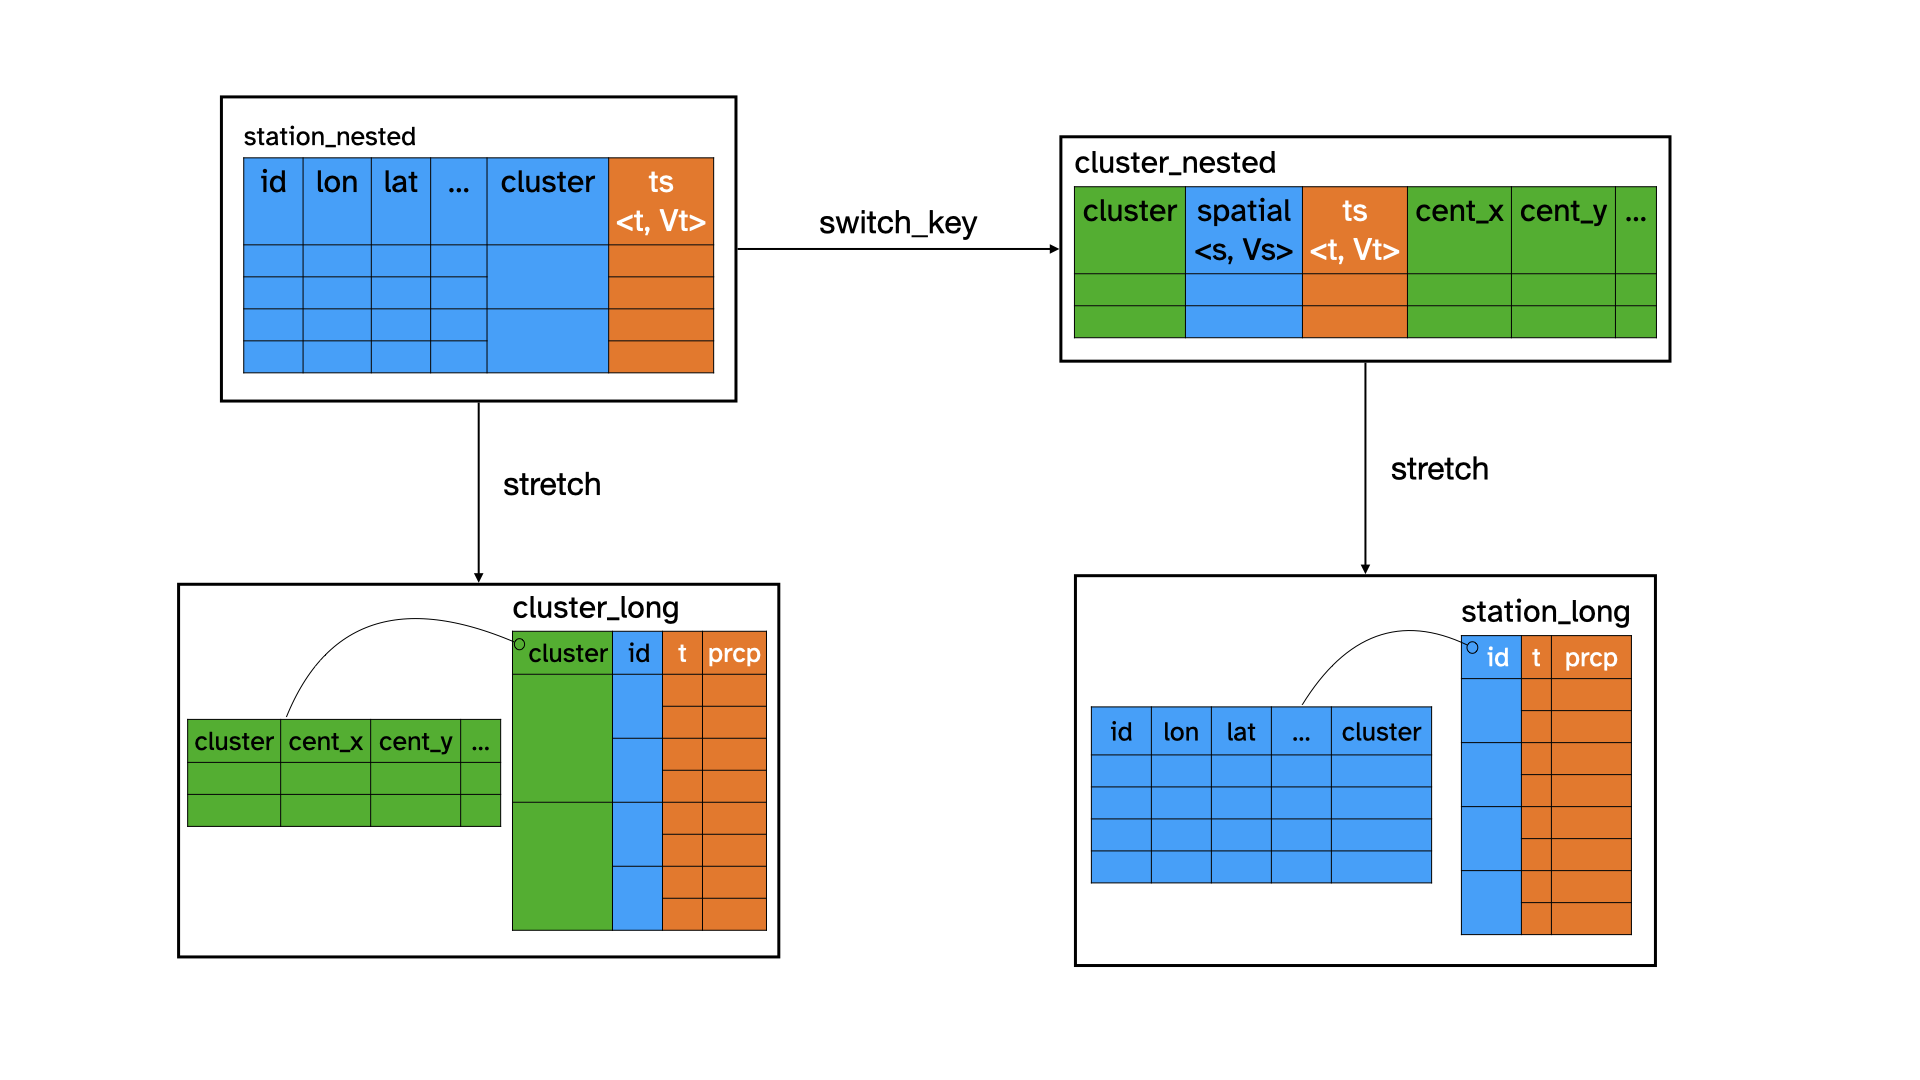
\includegraphics[width=1\linewidth,height=0.4\textheight]{/Users/sherryzhang/Documents/research/paper-cubble/figures/diagram-keynotes/diagram-keynotes.003} 

}

\caption[An illustration of the original and cluster level cubble in the nested form long form for hierarchical structure data]{An illustration of the original and cluster level cubble in the nested form long form for hierarchical structure data. \code{switch\_key()} changes the station level cubble into a cluster level cubble and both can be stretched into the long form.}\label{fig:illu-hier}
\end{figure}
\end{CodeChunk}

\hypertarget{data-fusion-and-matching}{%
\subsection{Data fusion and matching}\label{data-fusion-and-matching}}

One task that may interest analysts in spatio-temporal data is to find how similar the time series from nearby sites are. This can be seen as a matching problem \citep{stuart2010matching, mcintosh2018using} that pairs up similar similar time series in nearby locations or a data fusing exercise that merges data collected from different sources \citep{cocchi2019data}. \code{match_sites()} in \pkg{cubble} provides a simple algorithm for this task. The algorithm first matches the two data sources spatially through computing the pairwise distance on latitude and longitude. Pairs that pass the spatial matching are then matched temporally through computing the number of matched peaks within a fixed length window. Figure \ref{fig:illu-matching} illustrates this temporal matching in more details. Given two series \code{A} and \code{a}, 3 peaks have been picked in each series. An interval, with default length of 5, is constructed for each peak in series \code{A} and the peaks in series \code{a} are tested against whether they fall into the any of the intervals. In this illustration, there are 2 matches for these two series. Several arguments are available in \code{match_sites()} to fine-tune the matching:

\begin{CodeChunk}
\begin{figure}

{\centering 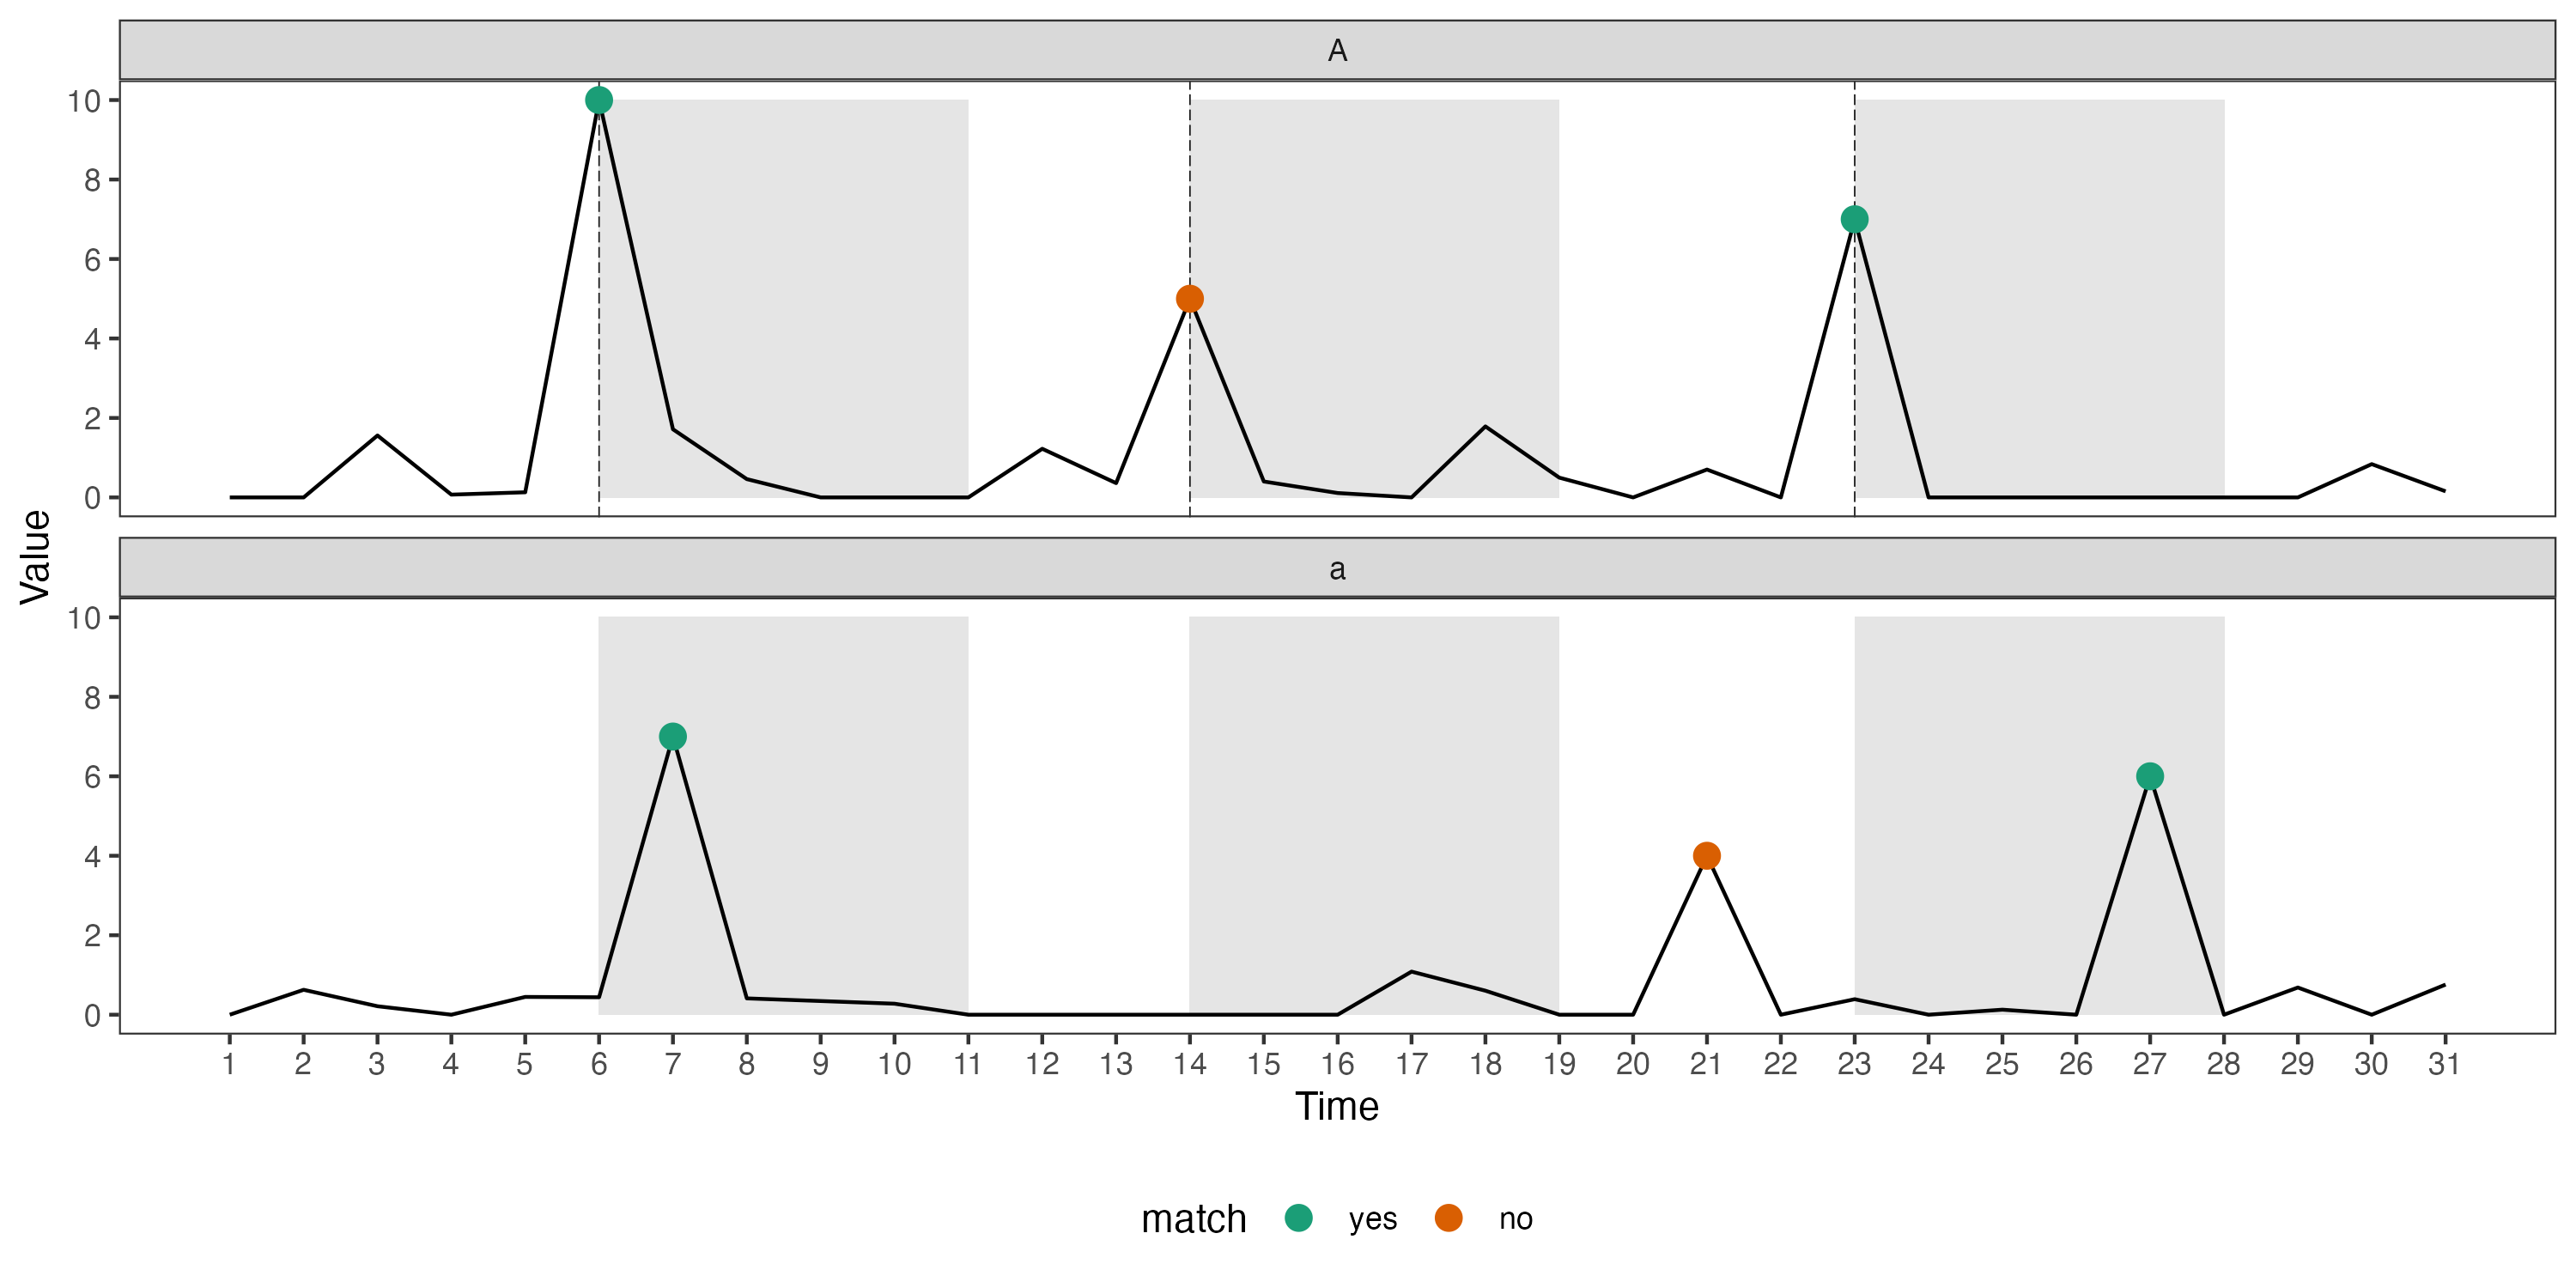
\includegraphics[width=1\linewidth]{/Users/sherryzhang/Documents/research/paper-cubble/figures/illu-matching} 

}

\caption{An illustration of temporal matching in cubble. Three highest peaks are identified in each series and intervals are constructed on series \code{A}. Two peaks in series \code{a} fall into the intervals and hence the two series are considered to have 2 matches.}\label{fig:illu-matching}
\end{figure}
\end{CodeChunk}

\begin{itemize}
\tightlist
\item
  \code{spatial_n_keep}: the number of spatial match for each site to keep
\item
  \code{spatial_dist_max}: the maximum distance allowed for a matched pair
\item
  \code{temporal_n_highest}: the number of peak used - 3 in the example above
\item
  \code{temporal_window}: the length of the interval - 5 in the example above
\item
  \code{temporal_min_match}: the minimum number of matched peak for a valid matched pair
\end{itemize}

\hypertarget{interactive-graphics}{%
\subsection{Interactive graphics}\label{interactive-graphics}}

Cubble fits in naturally with the interactive graphic pipeline discussed in the literature \citep{buja1988elements, buja1996interactive, sutherland2000orca, xie2014reactive, cheng2016enabling}. Diagram \ref{fig:illu-interactive} illustrates how linking works from the map to the time series in cubble. The map and time series plot is associated with the nested or long cubble, respectively, and when a user action is captured on the map, the site will be activated in the nested cubble (left). The nested cubble will communicate to the long cubble to activate all the observations with the same \code{id} (middle). The long cubble will then highlight the activated series in the time series plot (right).

The linking is also available from the time series plot to the map. The selection(s) on the time series is through selecting the point(s) on the time series and once a point is selected, it will be activated in the long cubble. All the observations that share the same \code{id} are then activated and this includes other points in the same time series in the long cubble and the corresponding observation of site in the nested cubble. These activated observations will then being reflected in the updated plots and Diagram \ref{fig:illu-interactive-2} in the Appendix illustrates this process.

\begin{CodeChunk}
\begin{figure}

{\centering 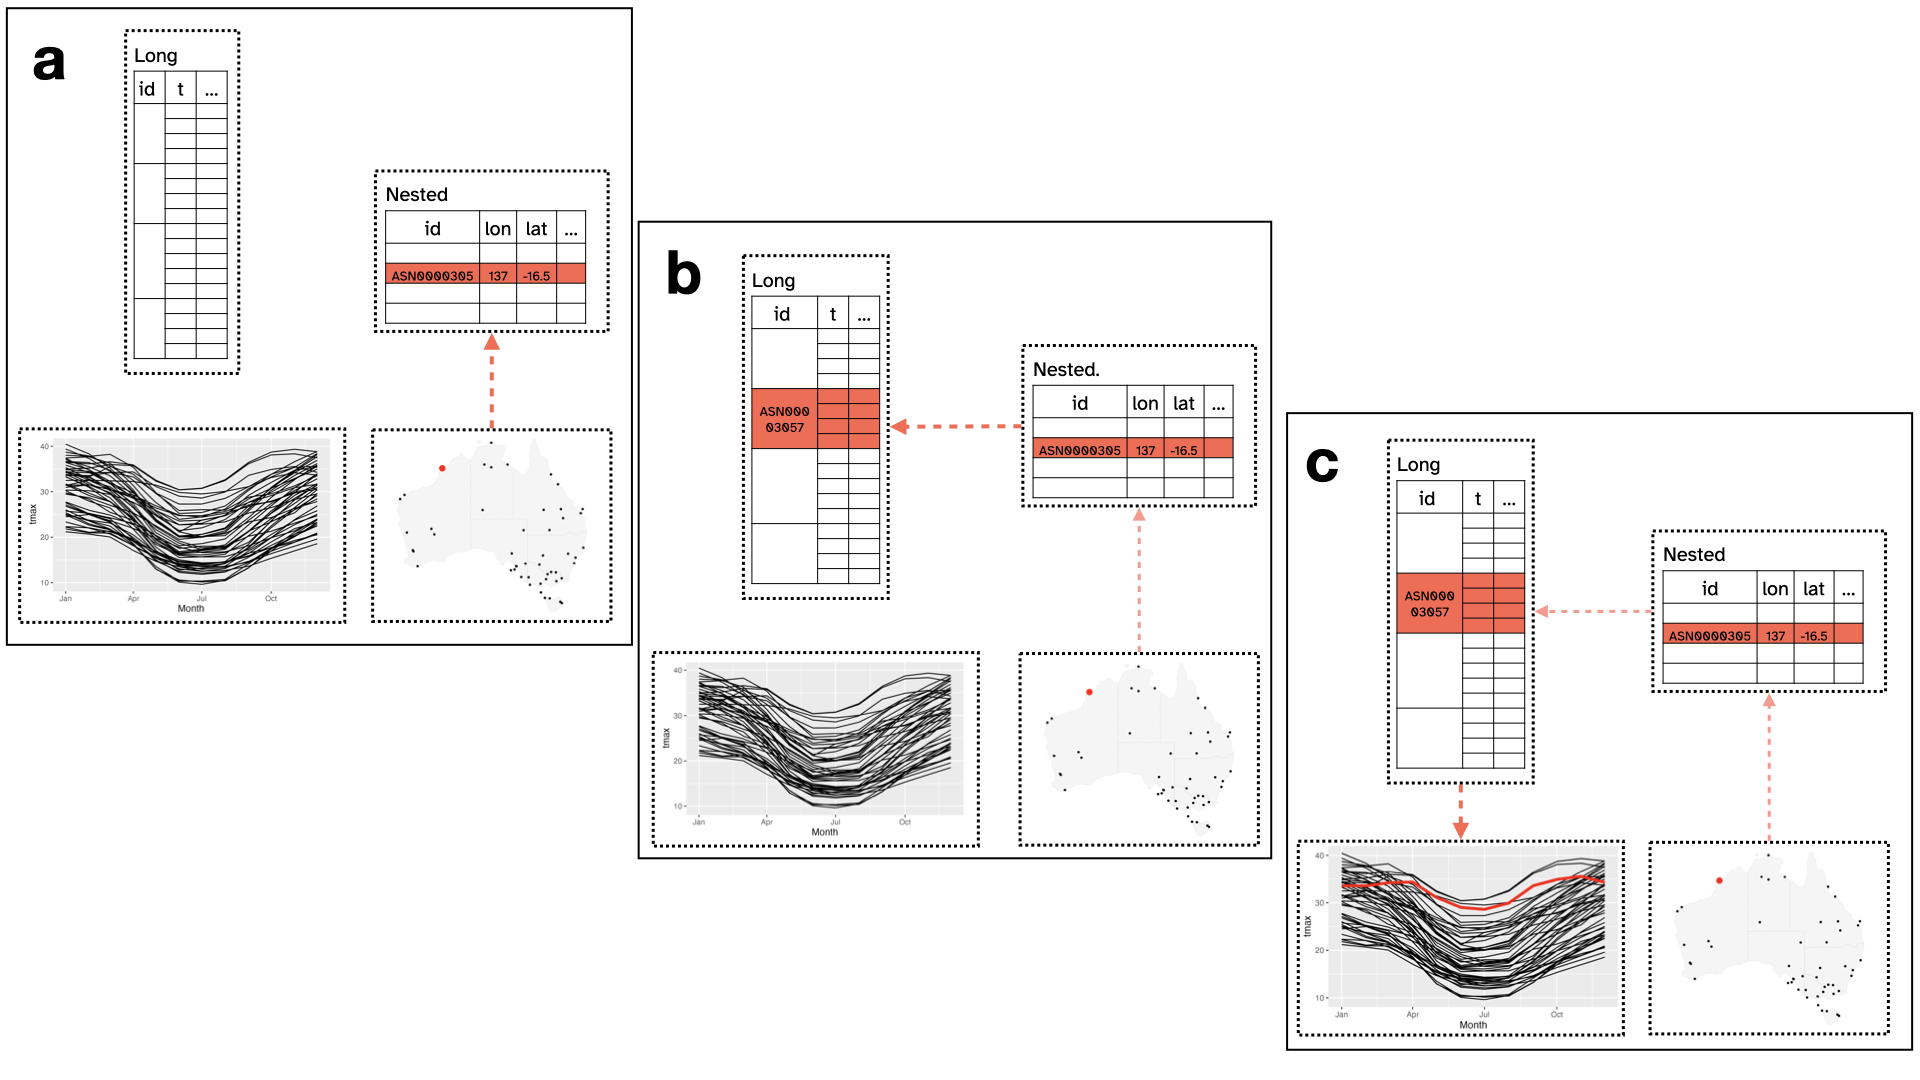
\includegraphics[width=1\linewidth,height=0.4\textheight]{/Users/sherryzhang/Documents/research/paper-cubble/figures/diagram-keynotes/diagram-keynotes.004} 

}

\caption[An illustration of the data model under interactive graphics with cubble]{An illustration of the data model under interactive graphics with cubble. The line plot and the map is made separately with the long and nested cubble. When a station is selected on the map (left), the corresponding row in the nested cubble will be activated. This will link to all the rows with the same id in the long cubble (middle) and update the line plot (right).}\label{fig:illu-interactive}
\end{figure}
\end{CodeChunk}

\hypertarget{st_transformation}{%
\subsection{Spatio-temporal transformations}\label{st_transformation}}

Spatio-temporal transformation is a useful technique to extract information form spatio-temporal data. Glyph maps \citep{Wickham2012-yr} transform the time coordinates into the space coordinates to plot the time series of different locations on the map. Calendar plots \citep{wang2020calendar} reconstructs time into calendar-based grid to discover weekday and weekend pattern. Projection, or linear combination, of variables summarises multivariate information into lower dimension to further digest. This section elaborates on the glyph map.

In \proglang{R}, \pkg{GGally} implements glyph maps through the \code{glyphs()} function. The function constructs a data frame with calculated position (\code{gx}. \code{gy}. \code{gid}) of each point on the time series using linear algebra (Equation 1 and 2 in \citet{Wickham2012-yr}). The data can then be piped into \code{ggplot} to create the glyph map as:

\begin{CodeChunk}
\begin{CodeInput}
R> library(ggplot2)
R> gly <- glyphs(data, 
+               x_major = ..., x_minor = ..., 
+               y_major = ..., y_minor = ..., ...)
R> 
R> ggplot(gly, aes(gx, gy, group = gid)) + 
+   geom_path() 
\end{CodeInput}
\end{CodeChunk}

A re-implementation of the glyph map as a ggproto, \code{GeomGlyph}, has been made in the \pkg{cubble} package and now the glyph map can be created with \code{geom_glyph()}:

\begin{CodeChunk}
\begin{CodeInput}
R> ggplot(data = data) +
+   geom_glyph(aes(x_major = ..., x_minor = ..., 
+                  y_major = ..., y_minor = ...))
\end{CodeInput}
\end{CodeChunk}

Some useful controls over the glyph map is also available in the \code{geom_glyph()} implementation. Polar glyph map can be specify as a parameter, \code{polar = TRUE}. in the \code{geom_glyph()}, along with \code{width} and \code{height} in either absolute or relative value. Global and local scale can be controlled by the parameter \code{global_rescale}. which default to \code{TRUE} for global scaling. Reference box and line can be added with separate \code{geom_glyph_box()} and \code{geom_glyph_line()}.

\hypertarget{examples}{%
\section{Examples}\label{examples}}

\hypertarget{covid}{%
\subsection{Victoria covid data}\label{covid}}

This example illustrate casting different sources into a cubble object. Victoria government of Australia provides daily COVID case number by date, source, and local government area (LGA). This data can be useful for visualising COVID spread when combined with LGA map information, which is available from Australian Bureau of Statistics. Variable \code{covid} and \code{lga} show the first 5 rows of these two data:

\begin{CodeChunk}
\begin{CodeInput}
R> covid |> head(5)
\end{CodeInput}
\begin{CodeOutput}
# A tsibble: 5 x 5 [1D]
# Key:       lga [1]
# Groups:    lga, source [1]
  date       lga        source                            n roll_mean
  <date>     <chr>      <chr>                         <int>     <dbl>
1 2022-01-01 Alpine (S) Contact with a confirmed case     1        NA
2 2022-01-02 Alpine (S) Contact with a confirmed case     2        NA
3 2022-01-03 Alpine (S) Contact with a confirmed case     4        NA
4 2022-01-04 Alpine (S) Contact with a confirmed case     4        NA
5 2022-01-05 Alpine (S) Contact with a confirmed case     2        NA
\end{CodeOutput}
\begin{CodeInput}
R> lga |> head(5)
\end{CodeInput}
\begin{CodeOutput}
Simple feature collection with 5 features and 7 fields
Geometry type: MULTIPOLYGON
Dimension:     XY
Bounding box:  xmin: 142.3643 ymin: -38.67876 xmax: 147.386 ymax: -36.39269
Geodetic CRS:  WGS 84
  lga_code_2018            lga state_code_2016 state_name_2016 areasqkm_2018
1         20110     Alpine (S)               2        Victoria     4788.1568
2         20260    Ararat (RC)               2        Victoria     4211.1171
3         20570   Ballarat (C)               2        Victoria      739.0321
4         20660    Banyule (C)               2        Victoria       62.5402
5         20740 Bass Coast (S)               2        Victoria      865.8095
  cent_long  cent_lat                       geometry
1  146.9742 -36.85357 MULTIPOLYGON (((146.7258 -3...
2  142.8432 -37.47271 MULTIPOLYGON (((143.1807 -3...
3  143.7815 -37.49286 MULTIPOLYGON (((143.6622 -3...
4  145.0851 -37.73043 MULTIPOLYGON (((145.1357 -3...
5  145.5581 -38.50730 MULTIPOLYGON (((145.5207 -3...
\end{CodeOutput}
\end{CodeChunk}

To cast these two data into a cubble object, supply them as a list with name \code{spatial} and \code{temporal} and other arguments (\code{key}, \code{index}, and \code{coords}). \code{as_cubble()} will automatically check the match of spatial and temporal information in the two datasets and warnings will emit if a location has missing spatial or temporal information.

\begin{CodeChunk}
\begin{CodeInput}
R> cb <- as_cubble(list(spatial = lga, temporal = covid),
+                 key = lga, index = date, coords = c(cent_long, cent_lat))
\end{CodeInput}
\begin{CodeOutput}
! Some sites in the temporal table don't have corresponding spatial information
\end{CodeOutput}
\begin{CodeOutput}
! Some sites in the spatial table don't have corresponding temporal information
\end{CodeOutput}
\begin{CodeOutput}
! Use argument `output = "unmatch"` to check on the unmatched key
\end{CodeOutput}
\end{CodeChunk}

Here, some locations have been detected with this issue and you can use \code{output = "unmatch"} to check on these locations:

\begin{CodeChunk}
\begin{CodeInput}
R> pair <- as_cubble(list(spatial = lga, temporal = covid),
+                 key = lga, index = date, coords = c(cent_long, cent_lat),
+                 output = "unmatch")
R> 
R> pair
\end{CodeInput}
\begin{CodeOutput}
$paired
# A tibble: 2 x 2
  spatial             temporal    
  <chr>               <chr>       
1 Kingston (C) (Vic.) Kingston (C)
2 Latrobe (C) (Vic.)  Latrobe (C) 

$others
$others$temporal
[1] "Interstate"       "Overseas"         "Queenscliffe (B)" "Unknown"         

$others$spatial
character(0)
\end{CodeOutput}
\end{CodeChunk}

\pkg{cubble} will make an attempt to pair the unmatched sites as well as showing unpaired locations. These can be useful information to help clean up the data.

\begin{CodeChunk}
\begin{CodeInput}
R> lga <- lga %>% 
+   mutate(lga = ifelse(lga == "Kingston (C) (Vic.)", "Kingston (C)", lga),
+          lga = ifelse(lga == "Latrobe (C) (Vic.)", "Latrobe (C)", lga)) %>%
+   filter(!lga %in% pair$others$spatial)
R> 
R> covid <- covid %>% filter(!lga %in% pair$others$temporal)
\end{CodeInput}
\end{CodeChunk}

After cleaning, you can cast the data into cubble with the same syntax without warnings:

\begin{CodeChunk}
\begin{CodeInput}
R> cb <- as_cubble(data = list(spatial = lga, temporal = covid),
+                 key = lga, index = date, coords = c(cent_long, cent_lat))
\end{CodeInput}
\end{CodeChunk}

\hypertarget{australia-historical-maximum-temperature}{%
\subsection{Australia historical maximum temperature}\label{australia-historical-maximum-temperature}}

Global Historical Climatology Network (GHCN) provides daily climate measures from stations across the world. The dataset \code{weatherdata::historical_tmax} extracts the maximum temperature for 236 Australian stations from GHCN with starting from year 1969. \code{weatherdata::historical_tmax} is already in a cubble, with \code{id} as the key, \code{date} as the index, and \code{c(longitude, latitude)} as the coordinates. This example compares the maximum temperature in two periods: 1971 - 1975 and 2016 - 2020 for stations in Victoria and New South Wales.

Stations in the two states can be subsetted by the station number: Australia GHCN station number starts with ``ASN00'' and followed by the \href{http://www.bom.gov.au/climate/cdo/about/site-num.shtml}{Bureau of Meteorology (BOM) station number}, where the 2nd and 3rd digit (7th and 8th in the GHCN number) define the state of the station. New South Wales stations start from 46 to 75 and Victoria stations follow from 76 to 90. Filtering Victoria and New South Wales stations is an operation in the spatial dimension and hence uses the nested form:

\begin{CodeChunk}
\begin{CodeInput}
R> tmax <- weatherdata::historical_tmax |>
+   filter(between(stringr::str_sub(id, 7, 8), 46, 90))
\end{CodeInput}
\end{CodeChunk}

Filtering for the period 1971 \textasciitilde{} 1975 and 2016 \textasciitilde{} 2020 is an operation on the time dimension and the nested cubble needs to be switched to the long cubble by \code{stretch()}:

\begin{CodeChunk}
\begin{CodeInput}
R> tmax <- tmax |> 
+   face_temporal() |>
+   filter(lubridate::year(date) %in% c(1971:1975, 2016:2020)) 
\end{CodeInput}
\end{CodeChunk}

A monthly average is used for both periods to smooth the maximum temperature and it is again an operation on the time dimension:

\begin{CodeChunk}
\begin{CodeInput}
R> tmax <- tmax |>
+   group_by(month = lubridate::month(date), 
+          group = as.factor(ifelse(lubridate::year(date) > 2015, 
+                                   "2016 ~ 2020", "1971 ~ 1975"))) |>
+   summarise(tmax = mean(tmax, na.rm = TRUE))
\end{CodeInput}
\end{CodeChunk}

A few stations don't have records during 1971 - 1975 and further investigation shows that while the first and last year of each series is recorded, the missing years in this period is not reported. These stations are filtered out by examining whether the summarised time series has a total of 24 months. The long cubble needs to be switched to the nested form for this spatial operation using \code{face_spatial()}:

\begin{CodeChunk}
\begin{CodeInput}
R> tmax <- tmax |> face_spatial() |> filter(nrow(ts) == 24) 
\end{CodeInput}
\end{CodeChunk}

Lastly, to create a glyph map, both the major (\code{longitude}, \code{latitude}) and minor (\code{month}, \code{tmax}) coordinates need to be in the same table. Spatial variables can be moved to the long form with \code{migrate()}:

\begin{CodeChunk}
\begin{CodeInput}
R> tmax <- tmax |> face_temporal() |> unfold(latitude, longitude)
\end{CodeInput}
\end{CodeChunk}

\code{tmax} can then be supplied to \code{geom_glyph()} for the glyph map in Figure \ref{fig:basic-manip} with a station inset on the top left corner:

\begin{CodeChunk}
\begin{CodeInput}
R> nsw_vic <- ozmaps::abs_ste |> 
+   filter(NAME %in% c("Victoria", "New South Wales"))
R> 
R> ggplot() + 
+   geom_sf(data = nsw_vic, 
+           fill = "transparent", color = "grey", linetype = "dotted") + 
+   geom_glyph(data = tmax, 
+              aes(x_major = longitude, x_minor = month, 
+                  y_major = latitude, y_minor = tmax,
+                  group = interaction(id, group), color = group),
+              width = 1, height = 0.5) +
+   ...
\end{CodeInput}
\end{CodeChunk}

\begin{CodeChunk}
\begin{figure}

{\centering 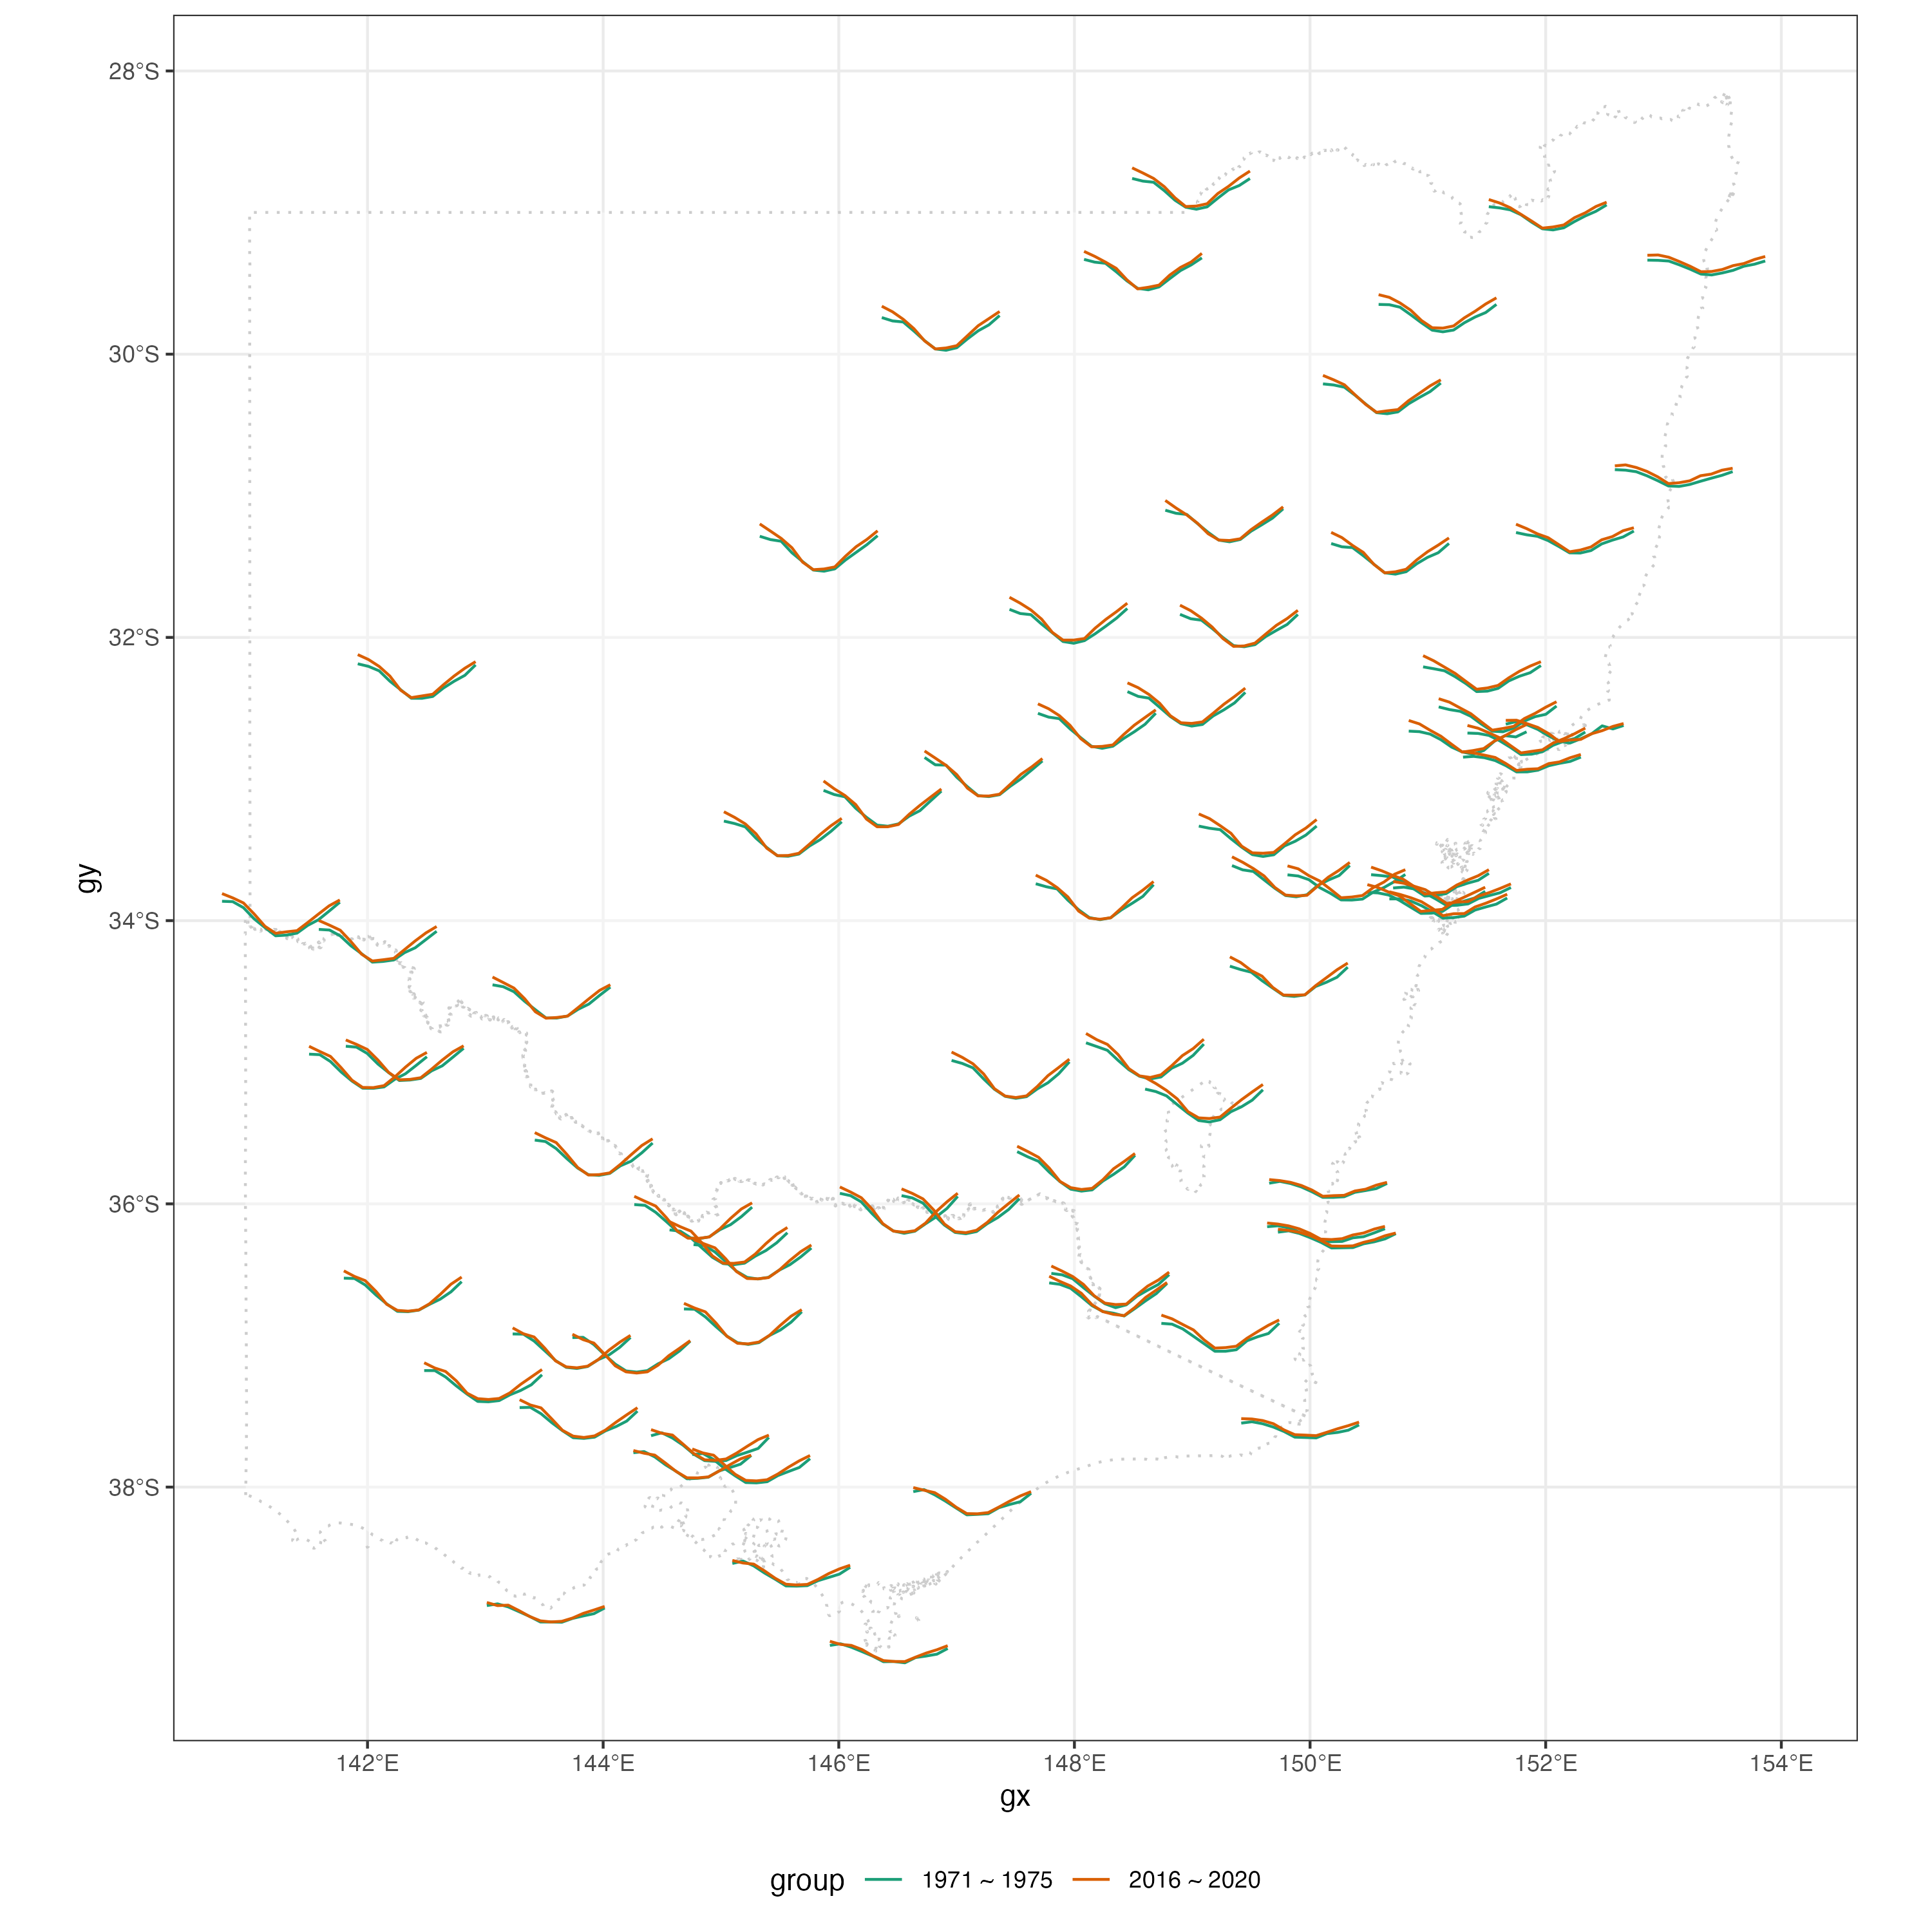
\includegraphics[width=1\linewidth,height=0.7\textheight]{/Users/sherryzhang/Documents/research/paper-cubble/figures/basic-manip} 

}

\caption[A glyph map of the average maximum temperature by month of Victoria and New South Wales weather stations in Australia]{A glyph map of the average maximum temperature by month of Victoria and New South Wales weather stations in Australia. On the top left corner is an insetted plot of station Cobar highlighted in the black box.}\label{fig:basic-manip}
\end{figure}
\end{CodeChunk}

\hypertarget{australia-precipitation-pattern-in-2020}{%
\subsection{Australia precipitation pattern in 2020}\label{australia-precipitation-pattern-in-2020}}

In the previous example, there has already been some overlapping of the glyphs for a few stations near (151E, 34S) and (152E, 33S) and this will be a problem when mapping more stations in the national level. Aggregation can be helpful to group series into clusters before visualising the cluster with glyph map. This example shows how to organise data at both level with \code{switch_key()}.

\code{weatherdata::climate_full}, also extracted from GHCN, records daily precipitation and maximum/ minimum temperature for 639 stations in Australia from 2016 to 2020. A simple kmean algorithm based on the distance matrix is used to create 20 clusters. This creates \code{station_nested} as a station level nested cubble with a cluster column indicating the group each station belongs to. More complex algorithms can be used for other problem, as long as there is a mapping from each station to a cluster.

\begin{CodeChunk}
\begin{CodeInput}
R> station_nested <- weatherdata::climate_full |> 
+   mutate(cluster = ...)
\end{CodeInput}
\end{CodeChunk}

To create a group level cubble, use \code{switch_key()} with the new key variable, \code{cluster}:

\begin{CodeChunk}
\begin{CodeInput}
R> cluster_nested <- station_nested |> switch_key(cluster) 
\end{CodeInput}
\end{CodeChunk}

With the group level cubble, \code{get_centroid()} is useful to compute the centroid of each cluster, which will be used as the major axis for the glyph map later:

\begin{CodeChunk}
\begin{CodeInput}
R> cluster_nested <- cluster_nested |> get_centroid()
\end{CodeInput}
\end{CodeChunk}

Long form cubble at both levels can be accessed through stretching the nested form and with access to both station and cluster level cubbles, various plots can be made to understand the cluster. Figure \ref{fig:basic-agg} shows two example plots that can be made with this data: subplot A is a glyph map made with the cluster level cubble in the long form and subplot B inspects the station membership of each cluster using the station level cubble in the nested form.

\begin{CodeChunk}
\begin{figure}

{\centering 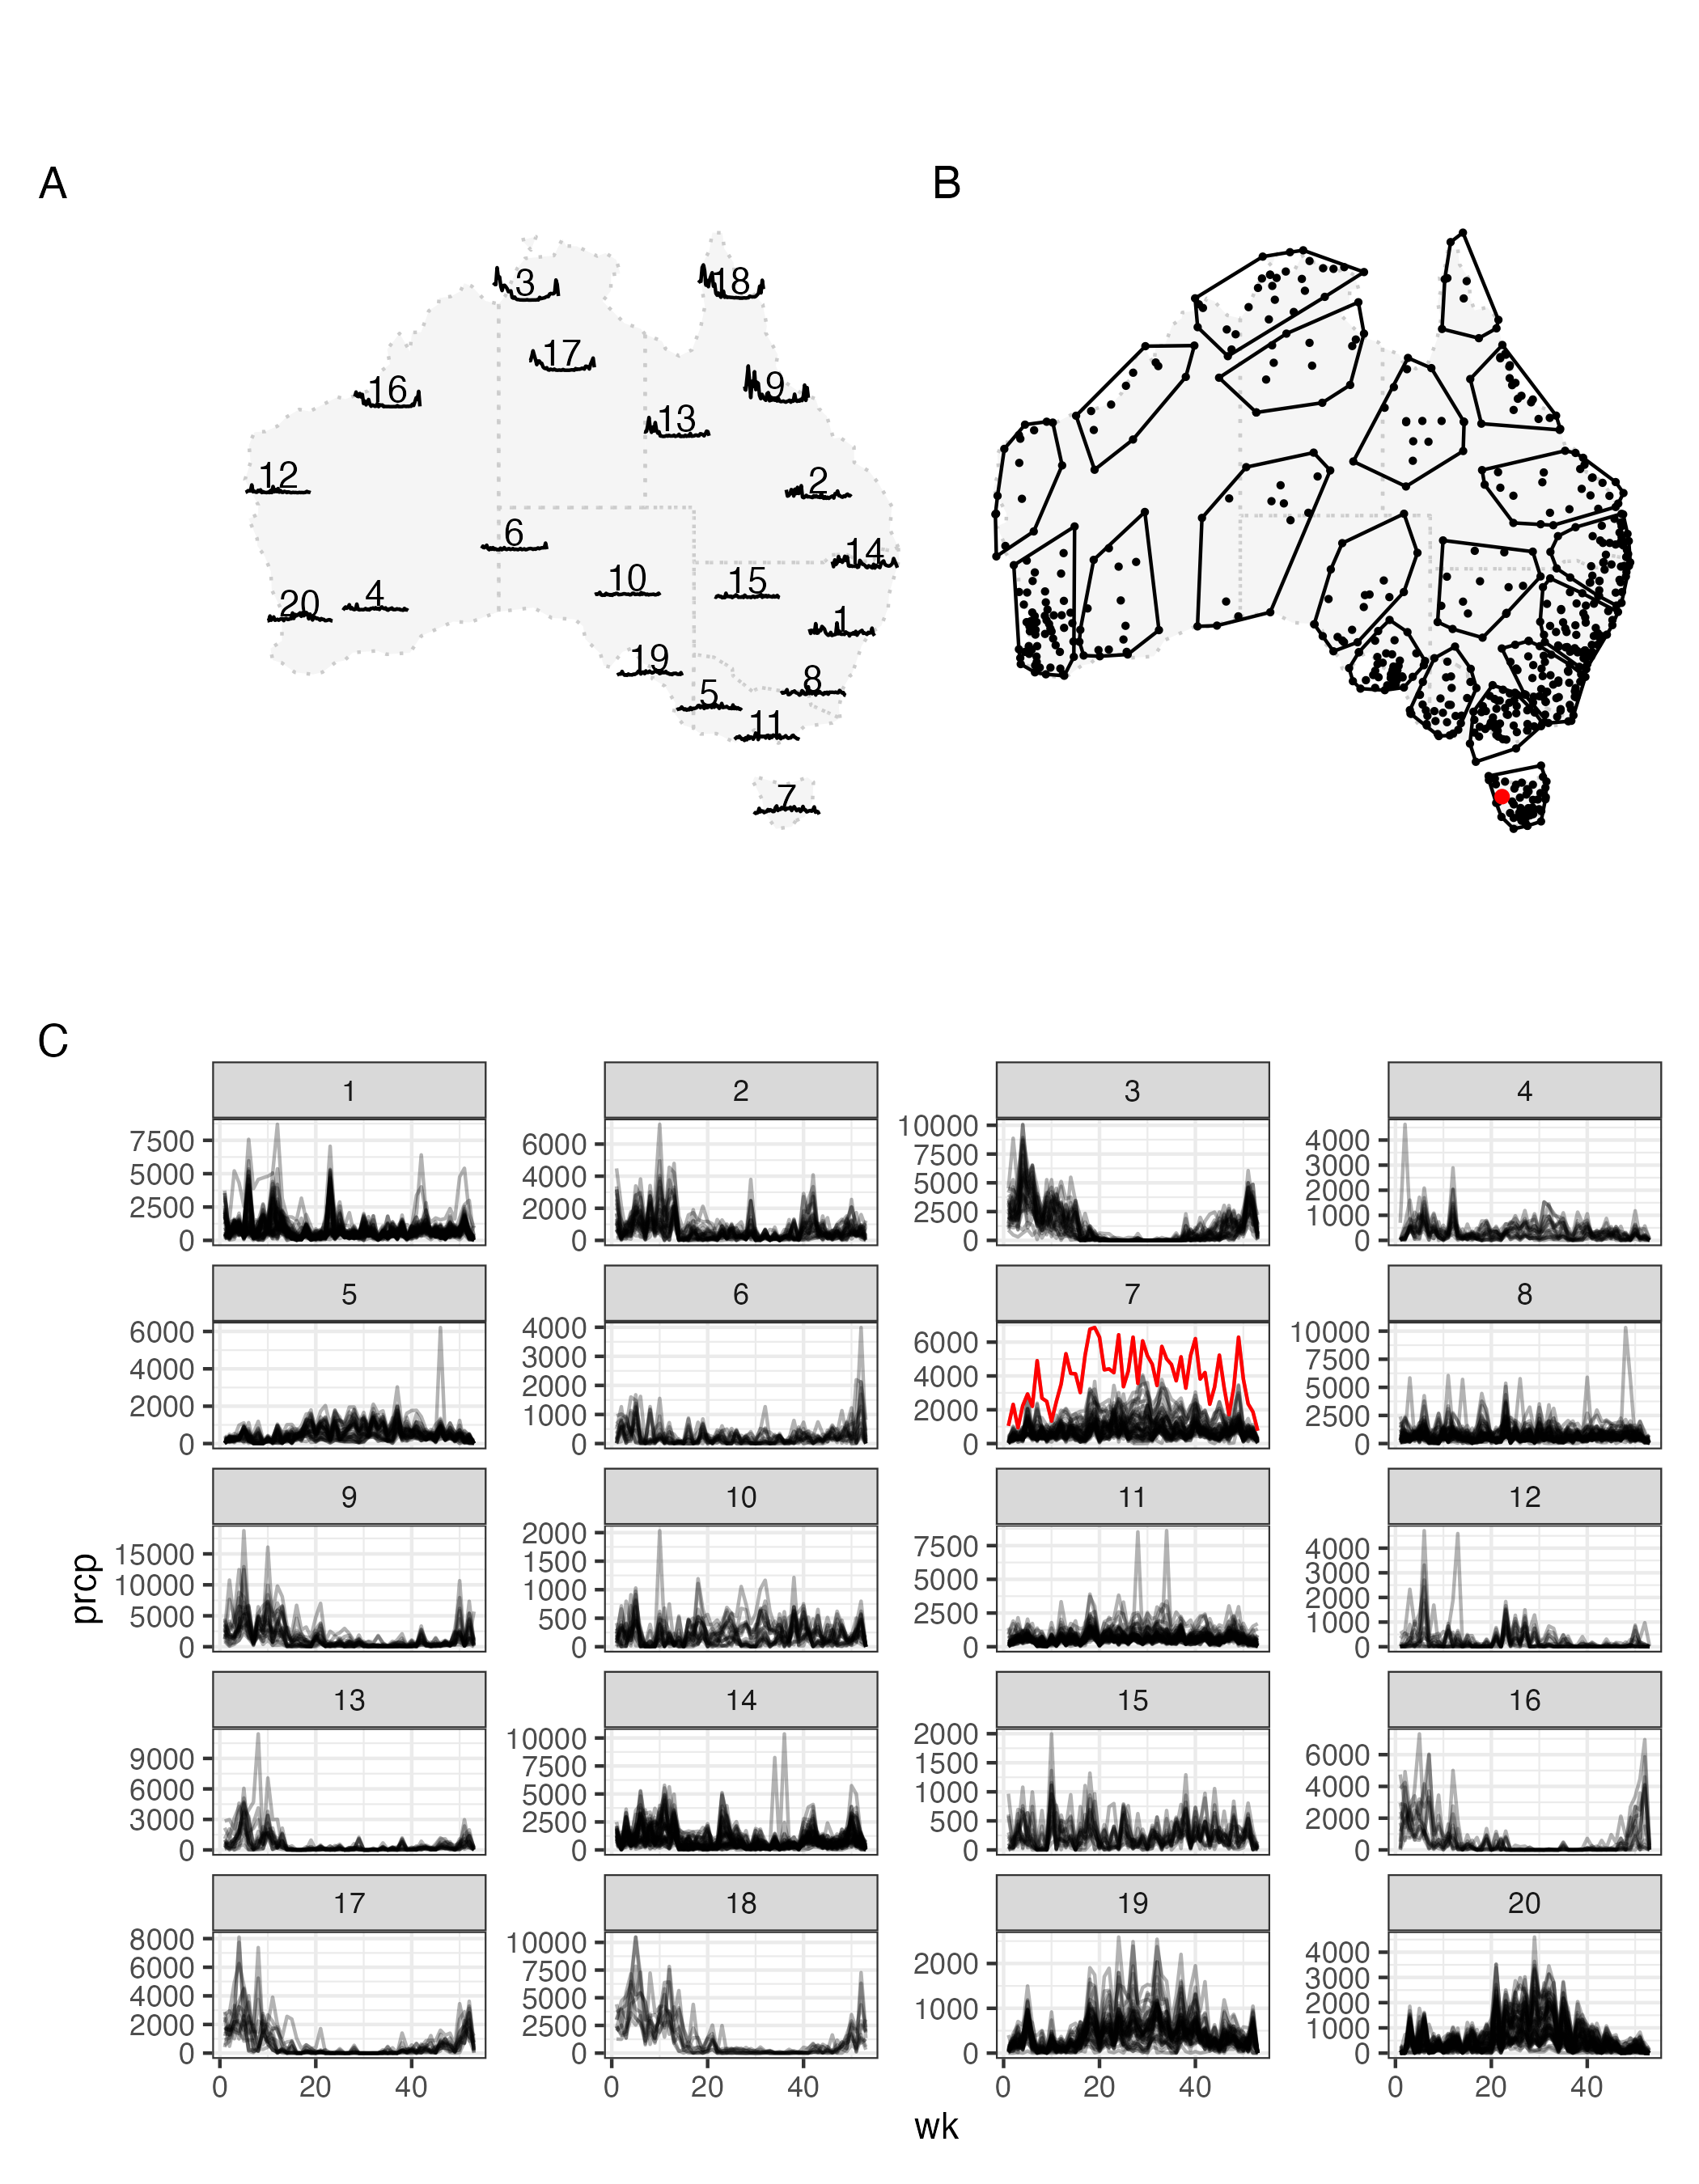
\includegraphics[width=1\linewidth]{/Users/sherryzhang/Documents/research/paper-cubble/figures/basic-agg} 

}

\caption[Profile of aggregated precipitation from 639 weather stations in Australia]{Profile of aggregated precipitation from 639 weather stations in Australia. Subplot A shows the glyph map of the weekly averaged precipitation of each cluster. The group number of printed in the middle of y minor axis and can be used as a reference line to read the magnitude. Subplot B shows the station membership of each cluster.}\label{fig:basic-agg}
\end{figure}
\end{CodeChunk}

\hypertarget{river-level-data-in-victoria-water-gauges}{%
\subsection{River level data in Victoria water gauges}\label{river-level-data-in-victoria-water-gauges}}

Bureau of Meteorology collects \href{http://www.bom.gov.au/metadata/catalogue/19115/ANZCW0503900528?template=full}{water data} from river gauges and this includes variables: electrical conductivity, turbidity, water course discharge, water course level, and water temperature. In particular, water level will interactive with precipitation from the climate data since rainfall will raise the water level in the river. Figure \ref{fig:matching-map} gives the location of available weather station and water gauges in Victoria.

\begin{CodeChunk}
\begin{figure}

{\centering 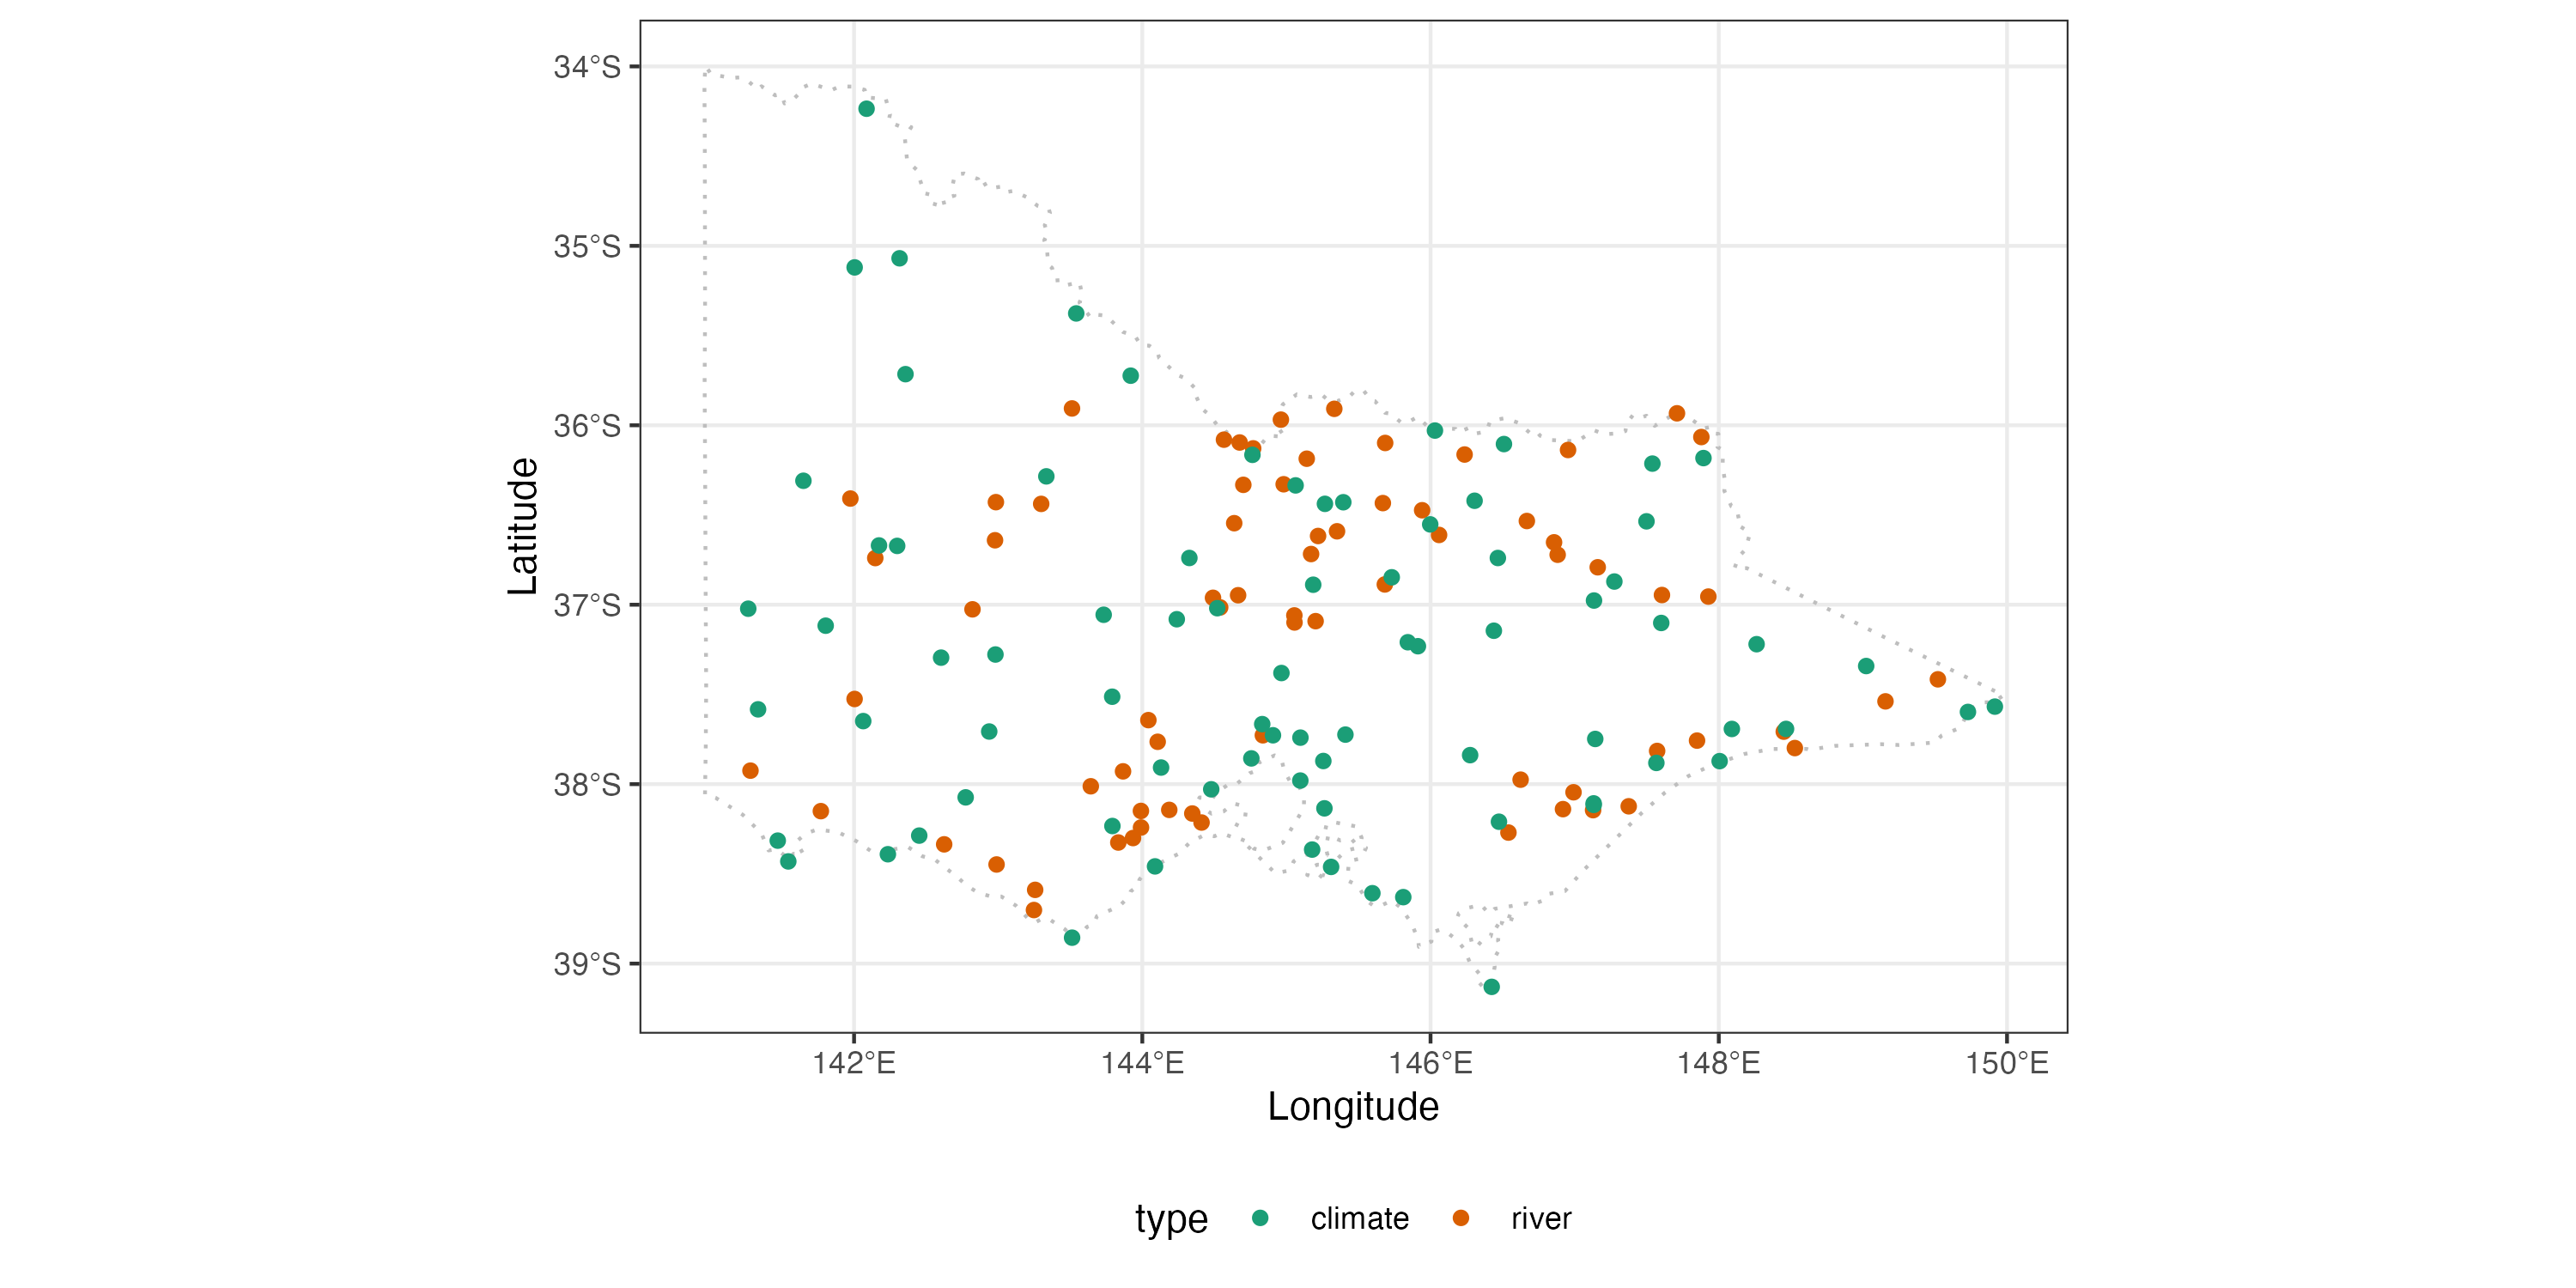
\includegraphics[width=1\linewidth]{/Users/sherryzhang/Documents/research/paper-cubble/figures/matching-map} 

}

\caption[Location of weather stations and river gauges in Victoria, Australia]{Location of weather stations and river gauges in Victoria, Australia.}\label{fig:matching-map}
\end{figure}
\end{CodeChunk}

From the map, a few water gauges and weather stations are close to each other and the fluctuation of the water level could be matched up with precipitation measured by the climate station. As introduced in Section 3.2, \code{match_sites()} can be used to match one source of data with another source in a cubble. Here \code{Water_course_level} in \code{river} will be matched to \code{prcp} in \code{climate} in 2020. The two datasets need to be specified as the first two arguments and the variable to match can be specified in \code{temporal_by} using the \code{by} syntax in \code{join}. \code{temporal_independent} controls the variable used to construct the interval and the goal here is to see if precipitation will be reflected by the water level in the river. This puts precipitation \code{prcp}, as the independent. Given there is one year worth of data, the number of peak (\code{temporal_n_highest}) to consider is slightly raised from a default 20 to 30 and \code{temporal_min_match} is raised accordingly To return all the pairs of the match, \code{temporal_min_match} can be set to 0.

\begin{CodeChunk}
\begin{CodeInput}
R> res <- match_sites(
+   river, climate,
+   temporal_by = c("Water_course_level" = "prcp"),
+   temporal_independent = "prcp",  
+   temporal_n_highest = 30,
+   temporal_min_match = 15
+ )
\end{CodeInput}
\end{CodeChunk}

The output from matching is also a cubble, with additional column \code{dist} and \code{group} produced from spatial matching and \code{n_match} from temporal matching.

\begin{CodeChunk}
\begin{CodeOutput}
# cubble:   id [8]: nested form
# bbox:     [144.52, -37.73, 146.06, -36.55]
# temporal: date [date], matched_var [dbl]
  id          name                  lat  long type   dist group ts       n_match
  <chr>       <chr>               <dbl> <dbl> <chr> <dbl> <int> <list>     <int>
1 405234      SEVEN CREEKS @ D/S~ -36.9  146. river  6.15     5 <tibble>      21
2 404207      HOLLAND CREEK @ KE~ -36.6  146. river  8.54    10 <tibble>      21
3 ASN00082042 strathbogie         -36.8  146. clim~  6.15     5 <tibble>      21
4 ASN00082170 benalla airport     -36.6  146. clim~  8.54    10 <tibble>      21
5 230200      MARIBYRNONG RIVER ~ -37.7  145. river  6.17     6 <tibble>      19
6 ASN00086038 essendon airport    -37.7  145. clim~  6.17     6 <tibble>      19
7 406213      CAMPASPE RIVER @ R~ -37.0  145. river  1.84     1 <tibble>      18
8 ASN00088051 redesdale           -37.0  145. clim~  1.84     1 <tibble>      18
\end{CodeOutput}
\end{CodeChunk}

Figure \ref{fig:matching} plots the matched pairs on the map or to view the matched series. There are four pairs of matches, which all locates in the middle Victoria and the concurrent increase of precipitation and water level can be observed.

\begin{CodeChunk}
\begin{figure}

{\centering 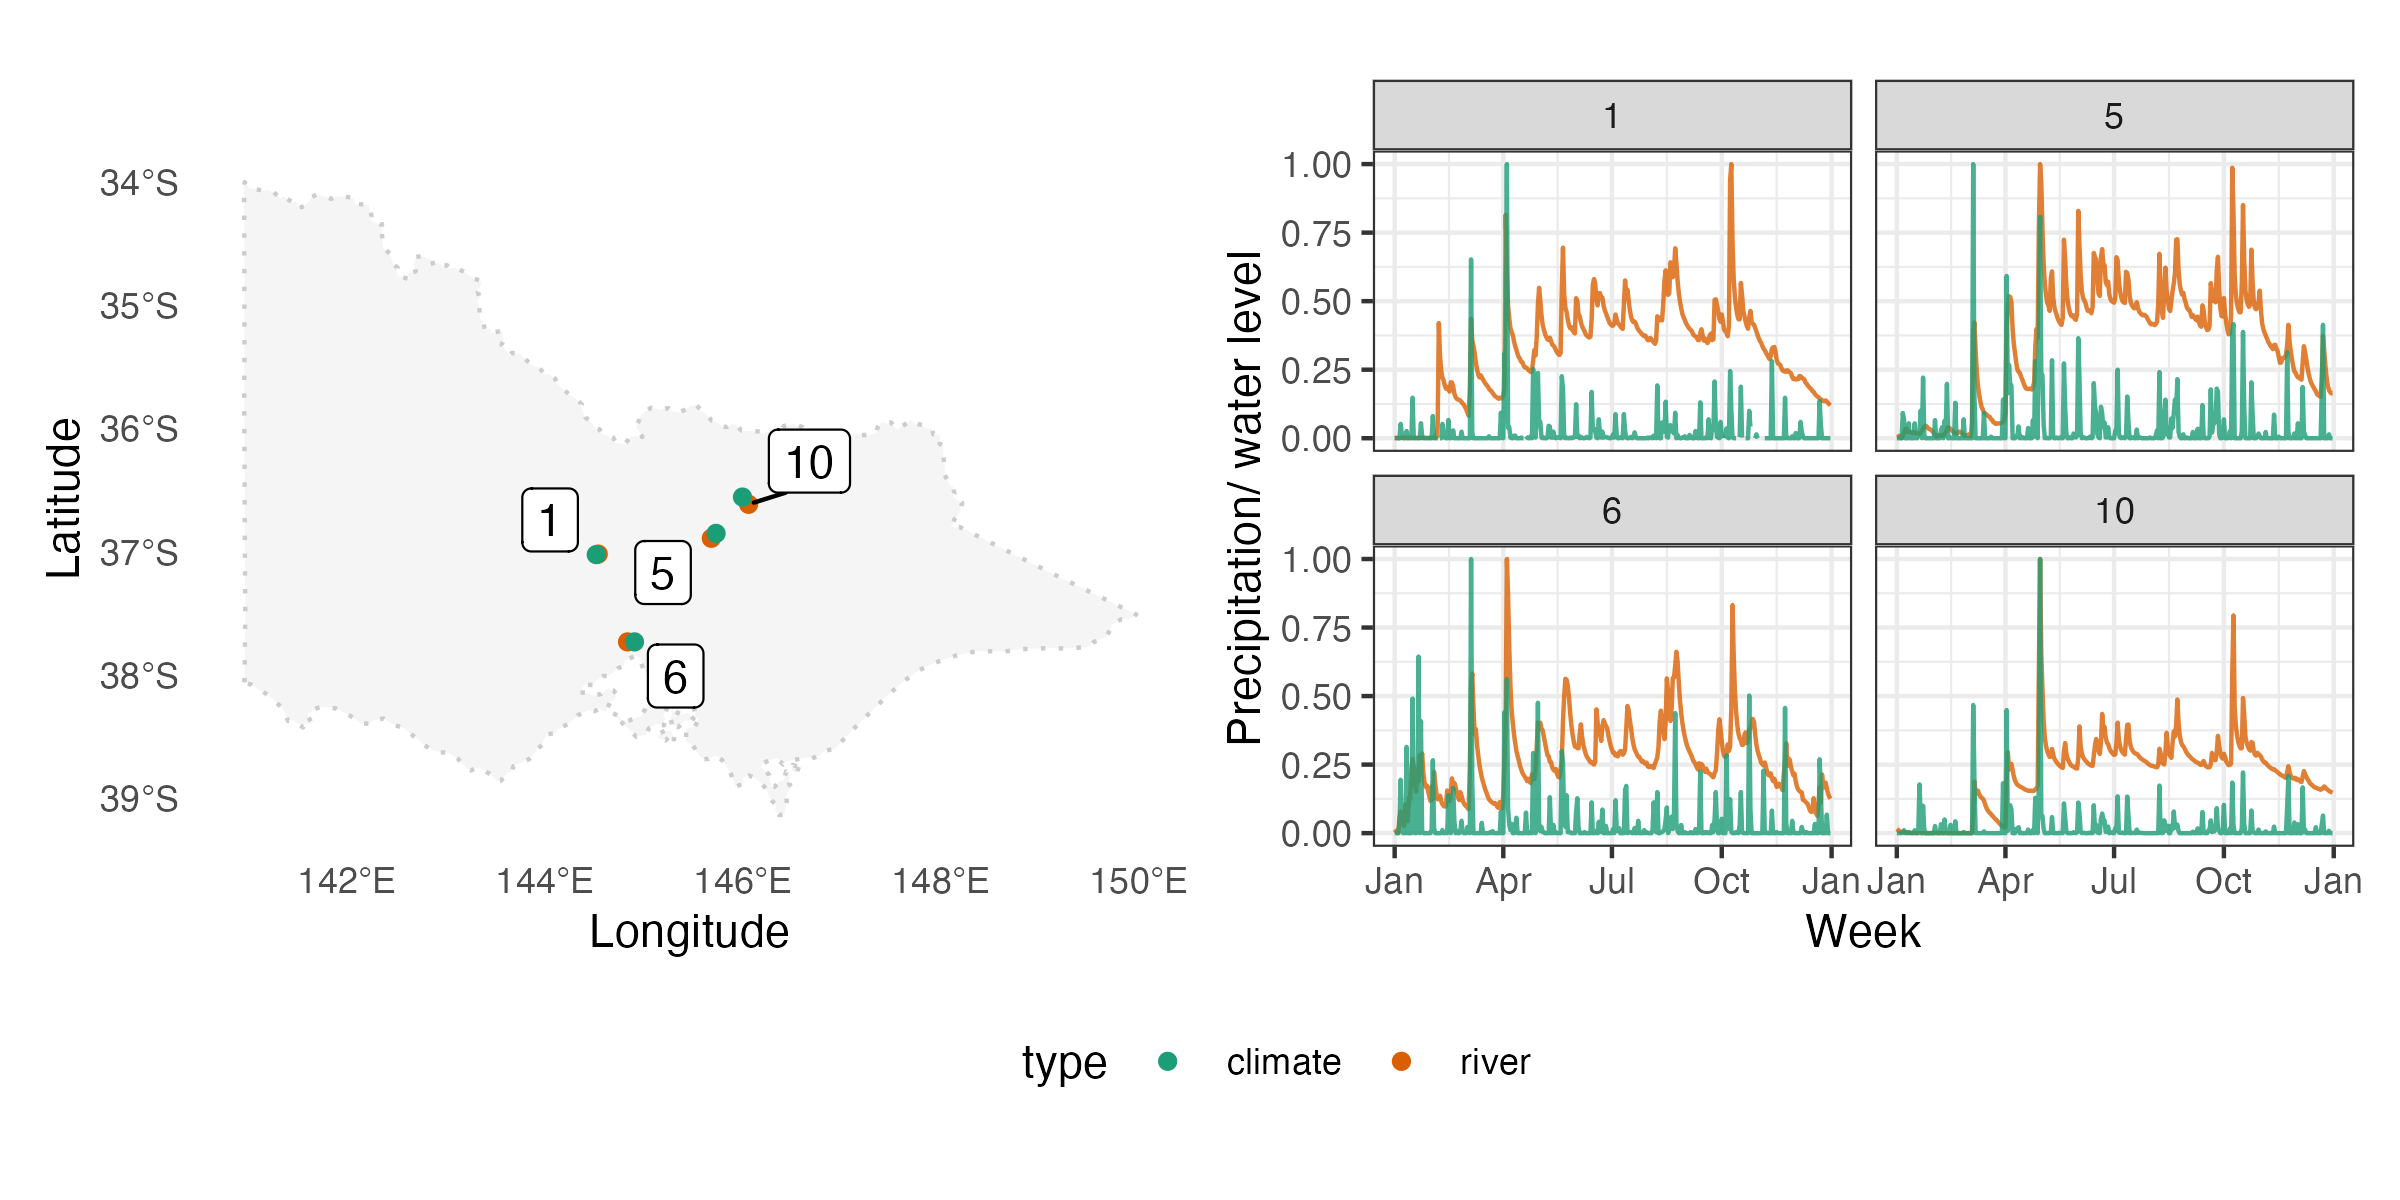
\includegraphics[width=1\linewidth]{/Users/sherryzhang/Documents/research/paper-cubble/figures/matching} 

}

\caption[Matched weather stations and river gauges on the map (A) and across time (B)]{Matched weather stations and river gauges on the map (A) and across time (B). Precipitation and water level have been standardised between 0 and 1 to be displayed on the same scale. The increases in the precipitation is reflected by the water level.}\label{fig:matching}
\end{figure}
\end{CodeChunk}

\hypertarget{era5-climate-reanalysis-data}{%
\subsection{ERA5: climate reanalysis data}\label{era5-climate-reanalysis-data}}

ERA5 data \citep{hersbach2020era5} is the latest reanalysis of global atmosphere, land surface, and ocean waves from 1950 onwards and is available in the NetCDF format from European Centre for Medium-Range Weather Forecasts (ECMWF). The data can be directly downloaded from \href{https://cds.climate.copernicus.eu/cdsapp\#!/dataset/reanalysis-era5-pressure-levels?tab=overview}{Copernicus Climate Data Store (CDS)} website or programmatically via an R package \pkg{ecmwfr} \citep{ecwmfr}. The \code{era5-pressure} data contains variable \emph{specific humidity} and \emph{geopotential} on the 10 hPa pressure level on four dates: 2002-09-22, 2002-09-26, 2002-09-30, and 2002-10-04. Once downloaded, the data can be read into a cubble as:

\begin{CodeChunk}
\begin{CodeInput}
R> raw <- ncdf4::nc_open(here::here("data/era5-pressure.nc"))
R> dt <- as_cubble(raw, vars = c("q", "z"))
\end{CodeInput}
\end{CodeChunk}

Figure \ref{fig:netcdf} reproduces the ERA5 data row of Figure 19 in \citet{hersbach2020era5}. It shows the southern polar vortex splits into two on 2002-09-26 and further splits into four on 2002-10-04 in the stratosphere. Readers interested in the analysis of this figure can refer to \citet{hersbach2020era5}, \citet{simmons2020global} and \citet{simmons2005ecmwf} for more details.

\begin{CodeChunk}
\begin{figure}

{\centering 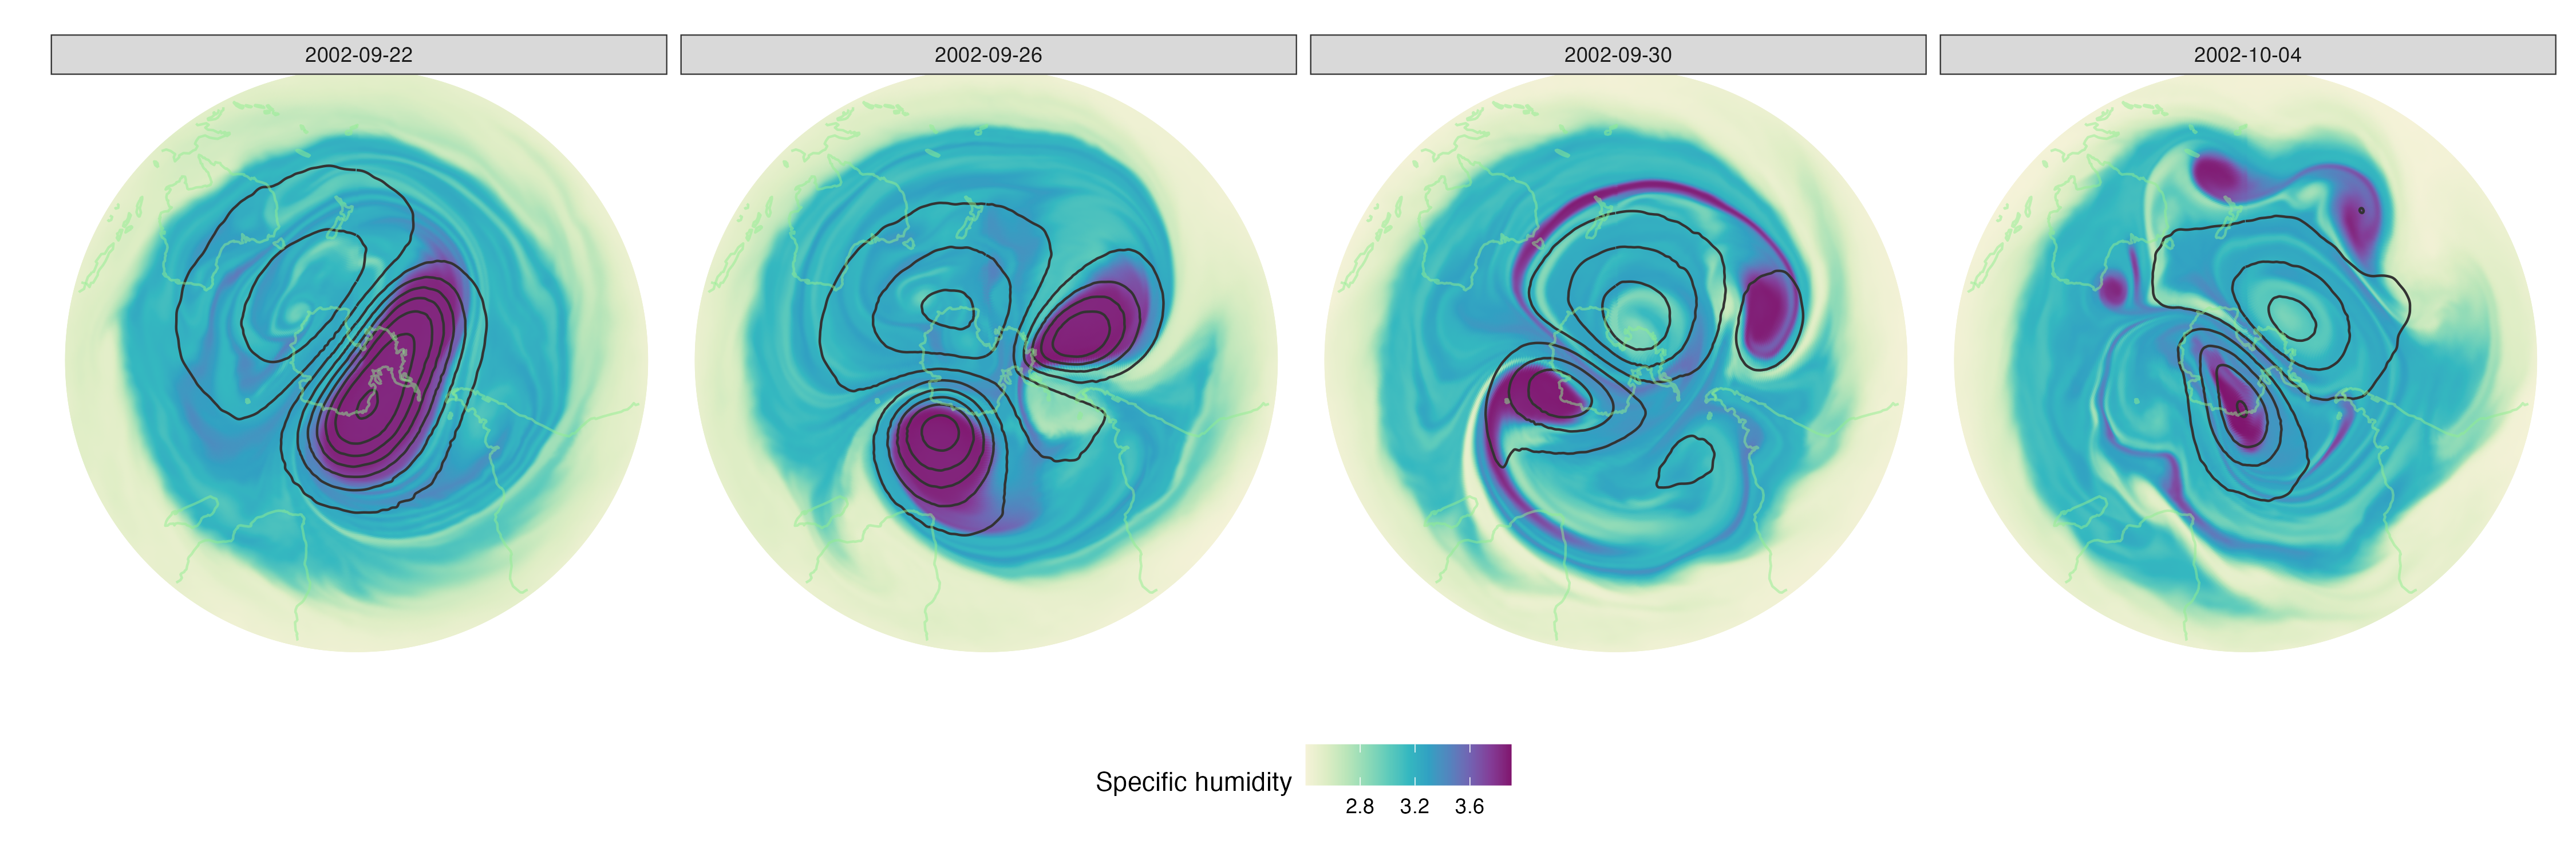
\includegraphics[width=1\linewidth]{/Users/sherryzhang/Documents/research/paper-cubble/figures/netcdf} 

}

\caption[A reproduction of the second row (ERA5 data) of Figure 19 in  Hersbach et al (2020)]{A reproduction of the second row (ERA5 data) of Figure 19 in  Hersbach et al (2020).}\label{fig:netcdf}
\end{figure}
\end{CodeChunk}

\hypertarget{interative-graphic}{%
\subsection{Interative graphic}\label{interative-graphic}}

With spatio-temporal data, users may wish to make plots to learn the spatial distribution of a variable, or to find patterns, such as trend or seasonality, in the time series. Combining this two types of plot with interactivity let users to link between points on the map and the corresponding time series to explore the spatial and temporal dimension of the data simultaneously. Below is an example that describes the process of building an interactive graphic with \pkg{cubble} and \pkg{crosstalk} The example explores the variation of monthly temperature range with \code{weatherdata::climate_full} data.

The temperature range is calculated as the difference between \code{tmax} and \code{tmin} and its monthly average over 2016 - 2020 is taken before calculating the variance. A \code{SharedData} object is constructed for each form of the cubble and the same \code{group} argument ensures the cross-linking of the two forms via the common \code{id} column. The spatial map and time series plot are then made with each \code{SharedData} objects separately. In this example, stations on the Australia map, made from the nested form, are coloured by the calculated variance and a ribbon band is constructed using the long form cubble to show the maximum and minimum temperature of each station across month. With a different dataset, users are free to calculate any per station measure in the nested form or to make any time-wise summary of the data in the long form to customise the spatial or temporal view. The cross-linking between the two plots is always safeguarded by the shared \code{id} column embedded in the cubble structure. Below is the pseudo code that outlines the process to construct an interactive graphic described above:

\begin{Shaded}
\begin{Highlighting}[]
\CommentTok{\# data pre{-}processing}
\NormalTok{clean }\OtherTok{\textless{}{-}}\NormalTok{ weatherdata}\SpecialCharTok{::}\NormalTok{climate\_full }\SpecialCharTok{|\textgreater{}}\NormalTok{ ...}

\CommentTok{\# created SharedData instance for crosstalk}
\NormalTok{nested }\OtherTok{\textless{}{-}}\NormalTok{ clean }\SpecialCharTok{|\textgreater{}}\NormalTok{ SharedData}\SpecialCharTok{$}\FunctionTok{new}\NormalTok{(}\SpecialCharTok{\textasciitilde{}}\NormalTok{id, }\AttributeTok{group =} \StringTok{"cubble"}\NormalTok{)}
\NormalTok{long }\OtherTok{\textless{}{-}} \FunctionTok{face\_temporal}\NormalTok{(clean) }\SpecialCharTok{|\textgreater{}}\NormalTok{ SharedData}\SpecialCharTok{$}\FunctionTok{new}\NormalTok{(}\SpecialCharTok{\textasciitilde{}}\NormalTok{id, }\AttributeTok{group =} \StringTok{"cubble"}\NormalTok{)}

\CommentTok{\# create the spatial and temporal view each with a ShareData instance}
\NormalTok{p1 }\OtherTok{\textless{}{-}}\NormalTok{ nested }\SpecialCharTok{|\textgreater{}}\NormalTok{ ...}
\NormalTok{p2 }\OtherTok{\textless{}{-}}\NormalTok{ long }\SpecialCharTok{|\textgreater{}}\NormalTok{ ...}

\CommentTok{\# Combine p1 and p2}
\NormalTok{crosstalk}\SpecialCharTok{::}\FunctionTok{bscols}\NormalTok{(plotly}\SpecialCharTok{::}\FunctionTok{ggplotly}\NormalTok{(p1), plotly}\SpecialCharTok{::}\FunctionTok{ggplotly}\NormalTok{(p2), ...)}
\end{Highlighting}
\end{Shaded}

In Figure \ref{fig:interactive-linking}, the first row shows the initial view of the interactive graphic. On the map, most regions in Australia have low variance of temperature range while the north-west coastline, bottom of South Australia, and Victoria stands out with larger monthly changes. In the second row, Mount Elizabeth is selected on the map given its high variance colour on the initial map and this links to the ribbon on the right. The third row the lowest temperature in August and this corresponds to Thredbo AWS in the Victoria and New South Wales border. Another station in the Tasmania island is selected on the map to cross compare with Thredbo AWS.

\begin{CodeChunk}
\begin{figure}

{\centering 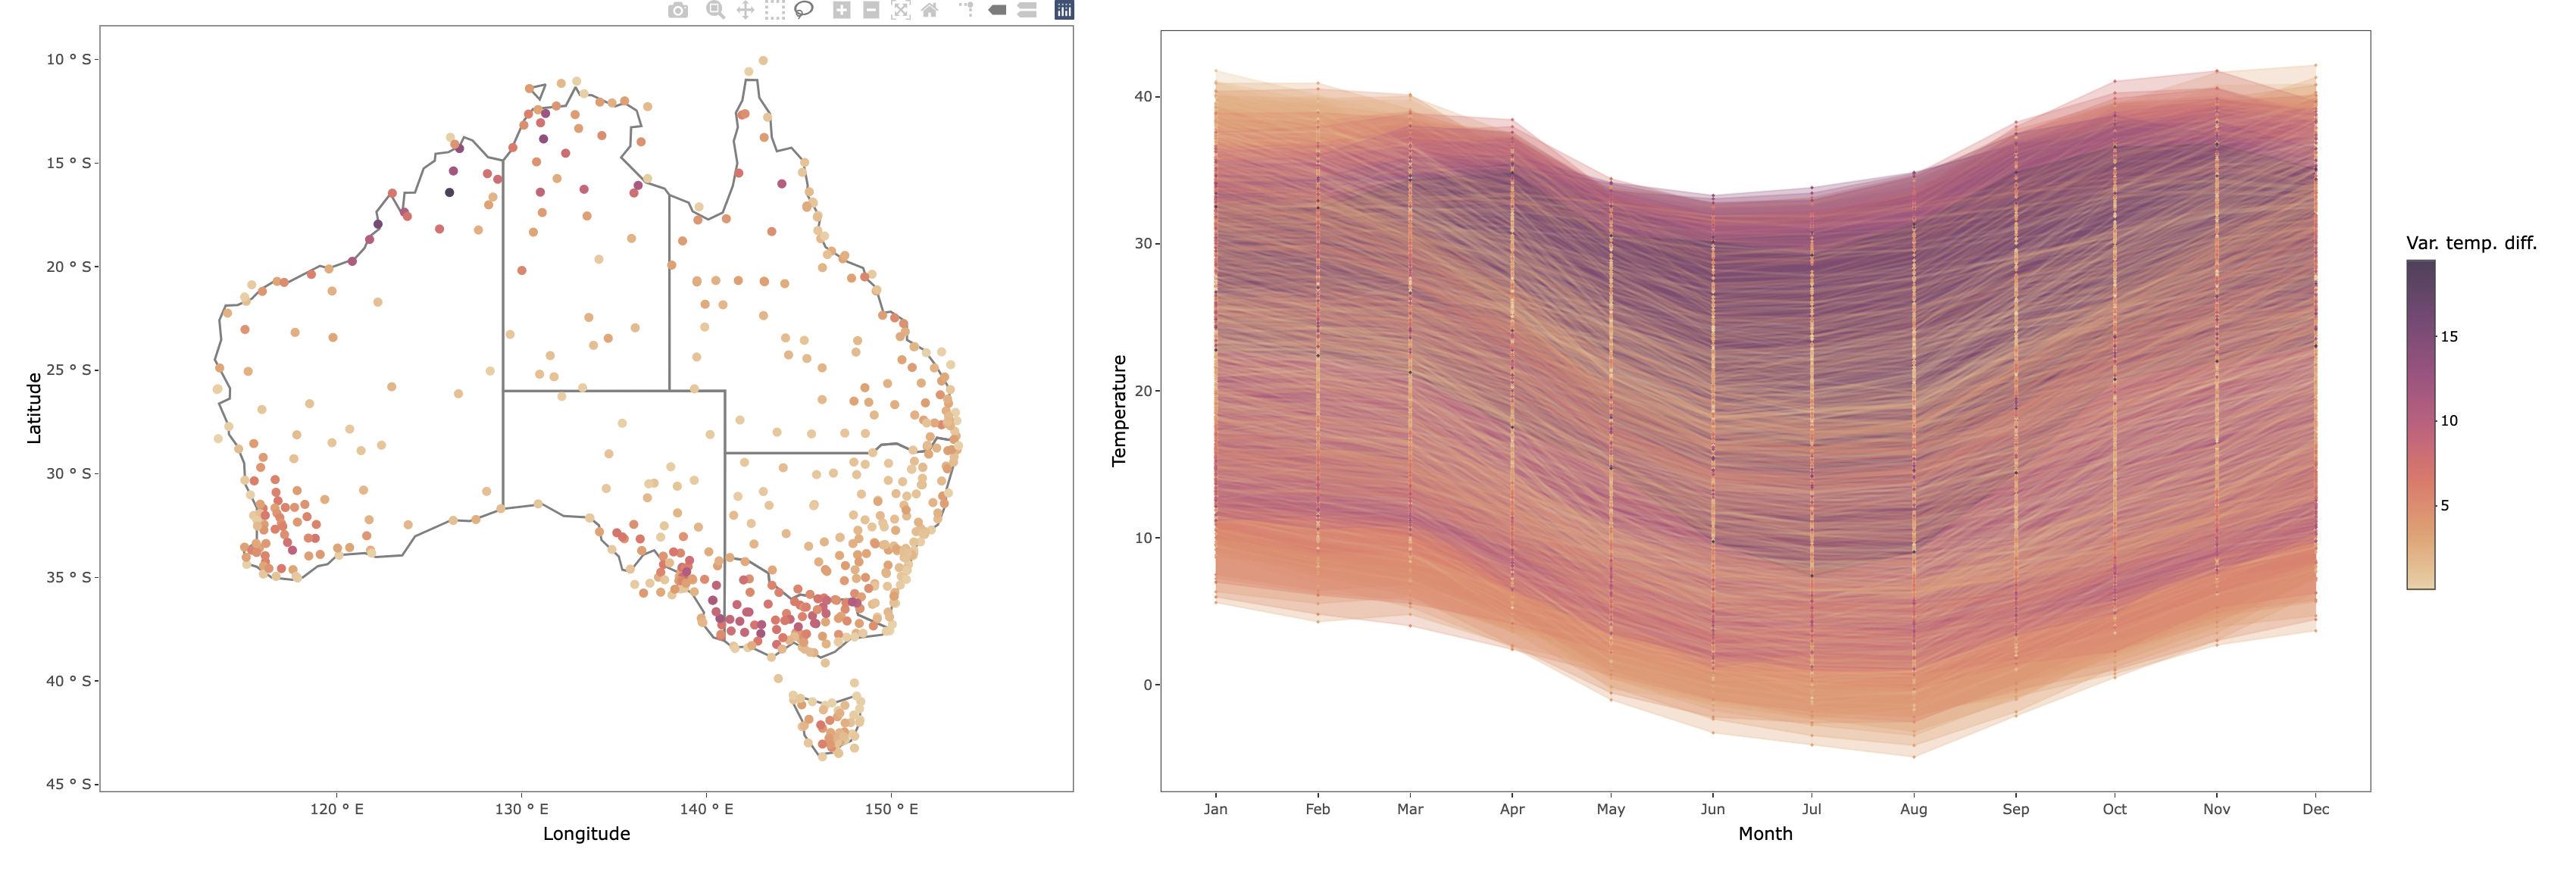
\includegraphics[width=1\linewidth,height=0.23\textheight]{/Users/sherryzhang/Documents/research/paper-cubble/figures/linking} 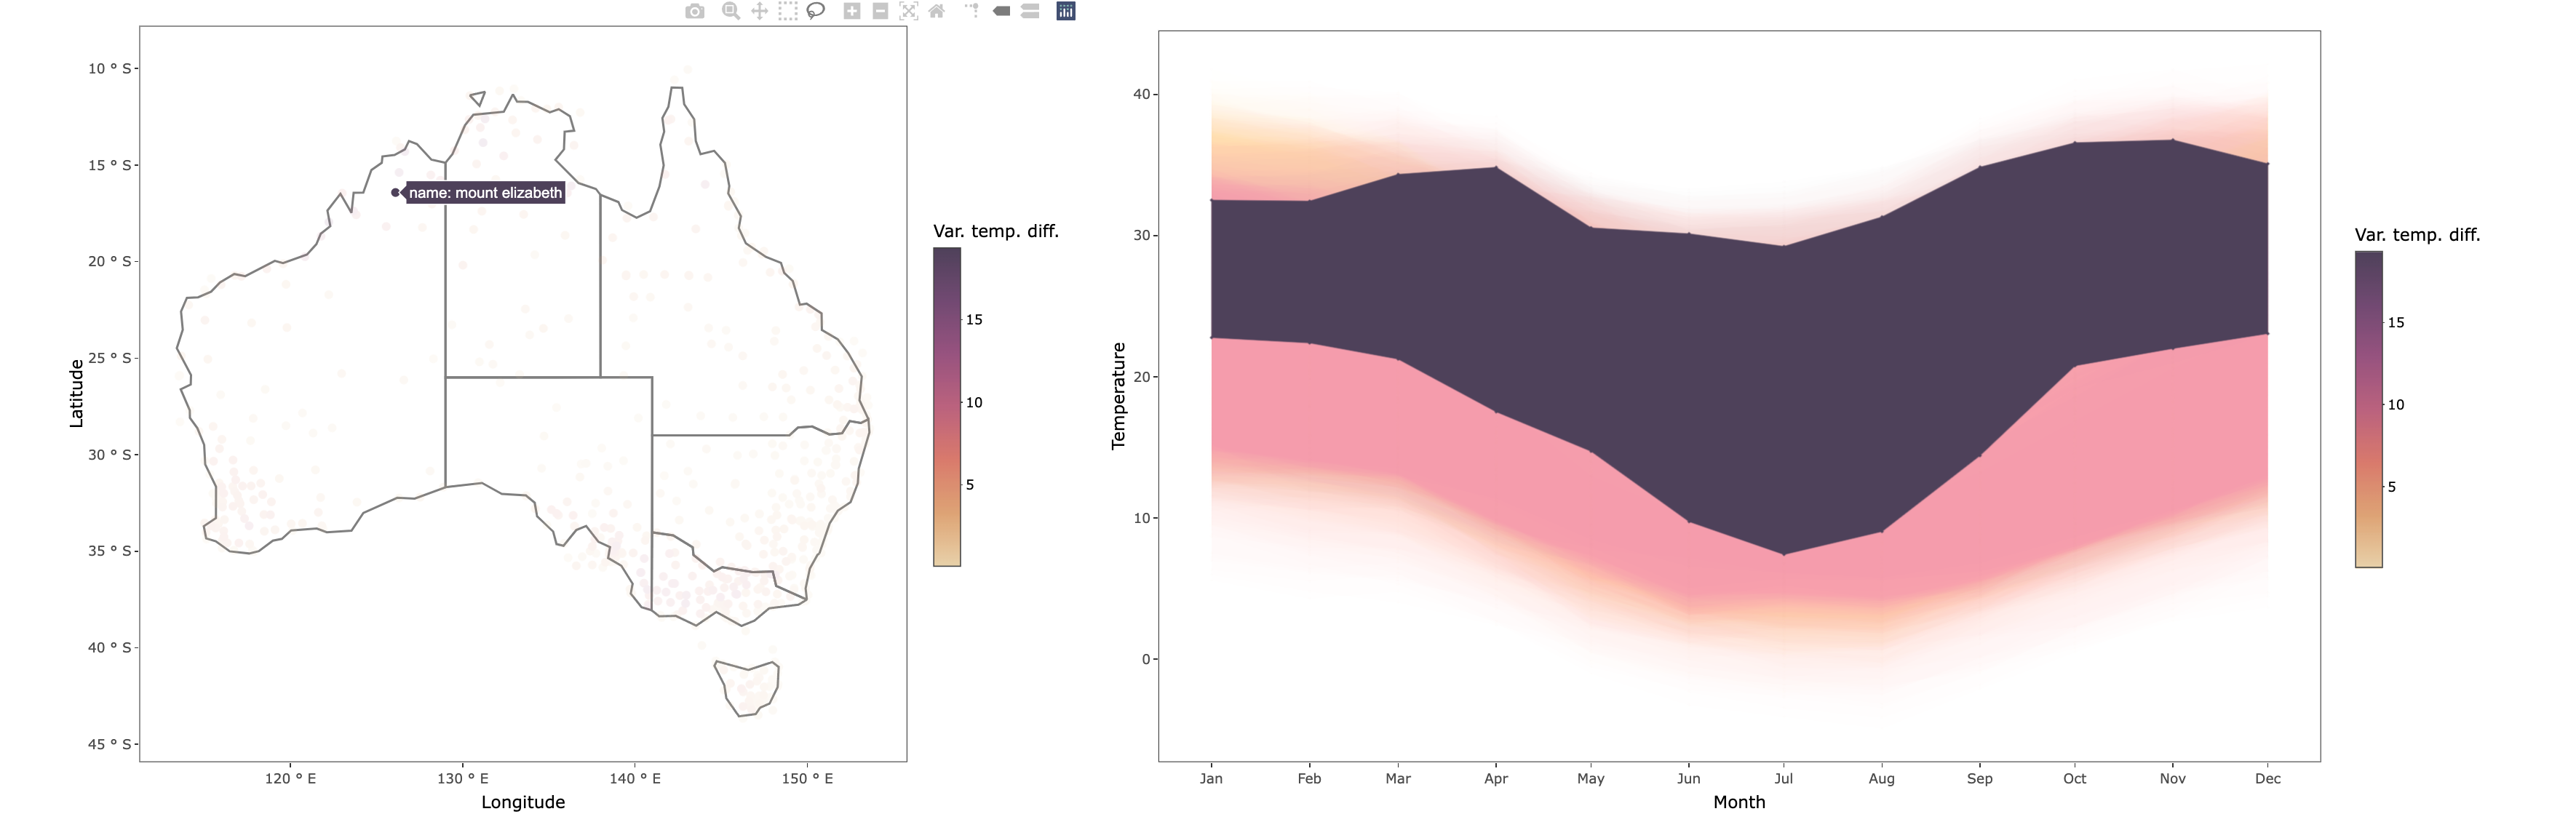
\includegraphics[width=1\linewidth,height=0.23\textheight]{/Users/sherryzhang/Documents/research/paper-cubble/figures/linking-north} 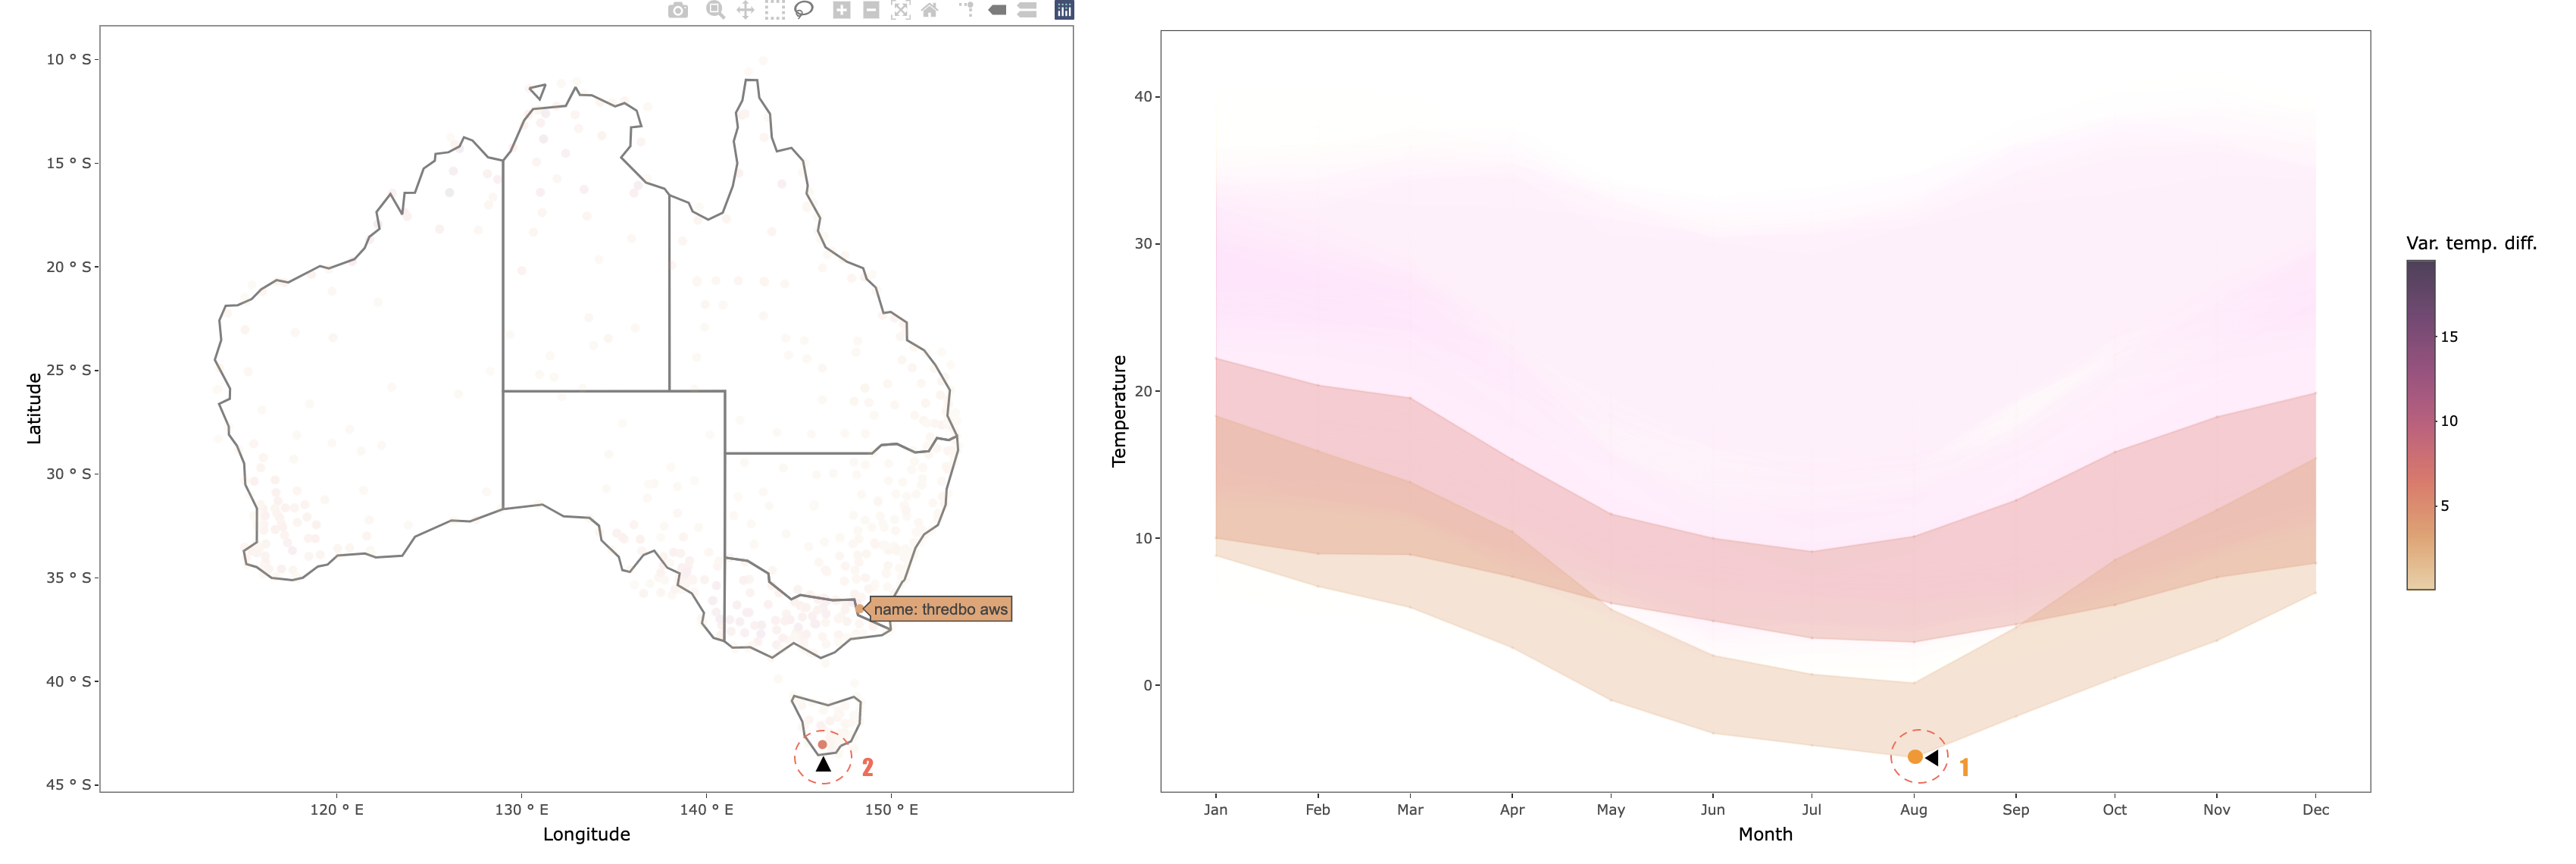
\includegraphics[width=1\linewidth,height=0.23\textheight]{/Users/sherryzhang/Documents/research/paper-cubble/figures/linking-lower} 

}

\caption[Exploring temperature variation using linking of a map and seasonal display]{Exploring temperature variation using linking of a map and seasonal display. Each row is a screen dump of the process. The top row shows all locations and all temperature profiles. Selecting a location with high variance on the map produces the plot in the second row. The maximum nad minimum temperature is shown using a ribbon. The bottom row first selects the lowest temperature in Auguest in the seasonal display. A location in the Tasmania Island is then selected to compare the temperature variation with Thredbo AWS.}\label{fig:interactive-linking}
\end{figure}
\end{CodeChunk}

This plot can also be made using \pkg{cubble} and \pkg{leaflet} where the temperature range can be displayed as a small subplot upon clicking on the map. This would require first creating the popup plots from the long form cubble as a vector and then add these plots to a leaflet map created from the nested cubble, with \code{leafpop::addPopupGraphs()}:

\begin{Shaded}
\begin{Highlighting}[]
\CommentTok{\# data pre{-}processing}
\NormalTok{clean }\OtherTok{\textless{}{-}}\NormalTok{ weatherdata}\SpecialCharTok{::}\NormalTok{climate\_full }\SpecialCharTok{|\textgreater{}}\NormalTok{ ...}

\CommentTok{\# use the long form to create subplots for each station}
\NormalTok{df\_id }\OtherTok{\textless{}{-}} \FunctionTok{unique}\NormalTok{(clean}\SpecialCharTok{$}\NormalTok{id)}
\NormalTok{p }\OtherTok{\textless{}{-}} \FunctionTok{map}\NormalTok{(}\DecValTok{1}\SpecialCharTok{:}\FunctionTok{length}\NormalTok{(df\_id), }\ControlFlowTok{function}\NormalTok{(i)\{}
\NormalTok{  dt }\OtherTok{\textless{}{-}}\NormalTok{ clean }\SpecialCharTok{|\textgreater{}} \FunctionTok{filter}\NormalTok{(id }\SpecialCharTok{==}\NormalTok{ df\_id[i])}
  \FunctionTok{ggplot}\NormalTok{(dt) }\SpecialCharTok{|\textgreater{}}\NormalTok{ ...}
\NormalTok{\})}

\CommentTok{\# create nested form leaflet map with temperature band as subplots}
\NormalTok{nested }\OtherTok{\textless{}{-}} \FunctionTok{face\_spatial}\NormalTok{(clean)}
\FunctionTok{leaflet}\NormalTok{(nested) }\SpecialCharTok{|\textgreater{}}
  \FunctionTok{addTiles}\NormalTok{() }\SpecialCharTok{|\textgreater{}}
  \FunctionTok{addCircleMarkers}\NormalTok{(}\AttributeTok{group =} \StringTok{"a"}\NormalTok{, ...) }\SpecialCharTok{|\textgreater{}}
\NormalTok{  leafpop}\SpecialCharTok{::}\FunctionTok{addPopupGraphs}\NormalTok{(}\AttributeTok{graph =}\NormalTok{ p, ...)}
\end{Highlighting}
\end{Shaded}

Figure \ref{fig:interactive-popup} shows Figure \ref{fig:interactive-linking} made made with leaflet and popups \citep{leafpop}.

\begin{CodeChunk}
\begin{figure}

{\centering 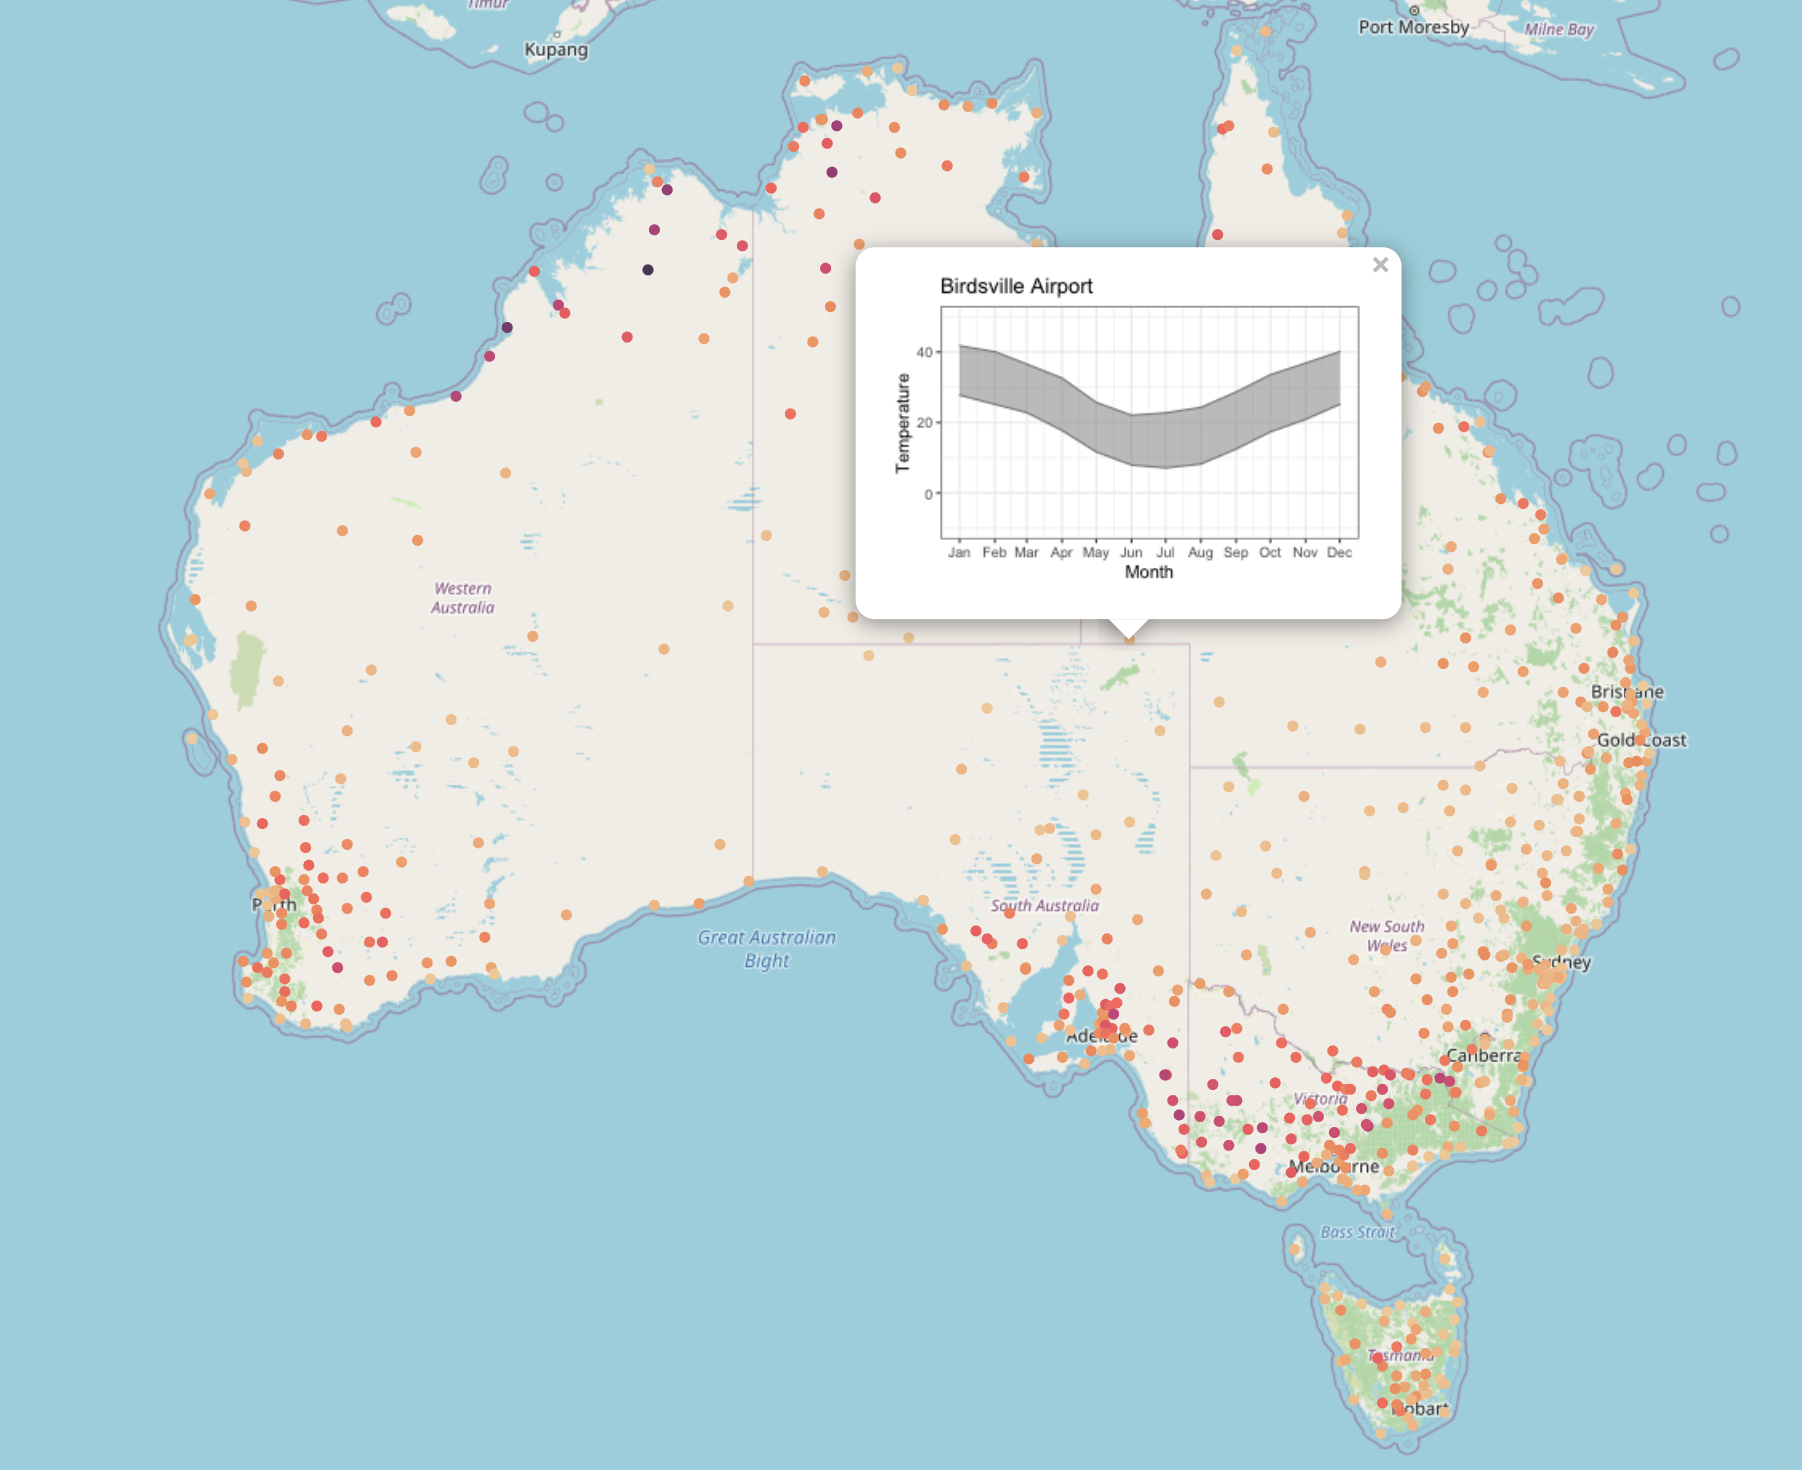
\includegraphics[width=0.45\linewidth,height=0.25\textheight]{/Users/sherryzhang/Documents/research/paper-cubble/figures/popup-mid} 

}

\caption[Same as Figure 11 with thetemperature variation shown as a popup in the leaflet map]{Same as Figure 11 with thetemperature variation shown as a popup in the leaflet map.}\label{fig:interactive-popup}
\end{figure}
\end{CodeChunk}

\hypertarget{conclude}{%
\section{Conclusion}\label{conclude}}

This paper describes an \proglang{R} package \pkg{cubble} for manipulating and visualising spatio-temporal data. A new data structure, \code{cubble} that builds from the \code{rowwise_df} and \code{grouped_df} class in the tidyverse ecosystem, is proposed to connect the time invariant and varying variables in the spatio-temporal data. This design frees the data analysts from spending time on organising variables of different observational units. The data structure is also flexible to the techniques and packages analysts use to analyse the data, for example, in the matching example in section 4.3, users are free to use algorithms from another package to cluster stations.

Further development and maintenance of the package involves responding to changes in the tidyverse packages that \pkg{cubble} imports, in particular, \pkg{tibble}, \pkg{tidyr}, and \pkg{dplyr}. In the spatial aspect, the simple feature representation wraps spatial coordinates in a list column, for some complex spatial operations, while sometimes, analysts may want to unpack them into longitude and latitude columns to work from. Another extension to \pkg{cubble} is to build a smooth transition between the coordinate columns and simple feature geometry column.

\newpage

\hypertarget{acknowledgement}{%
\section{Acknowledgement}\label{acknowledgement}}

This work is funded by the Commonwealth Scientific and Industrial Research Organisation (CSIRO) Data61 Scholarship and started while Nicolas Langrené was affiliated with CSIRO's Data61. The article is created using \pkg{knitr} \citep{knitr} and \pkg{rmarkdown} \citep{rmarkdown} in R. The source code for reproducing this paper can be found at: \url{https://github.com/huizezhang-sherry/paper-cubble}.

\hypertarget{appendix}{%
\section{Appendix}\label{appendix}}

\begin{CodeChunk}
\begin{figure}

{\centering 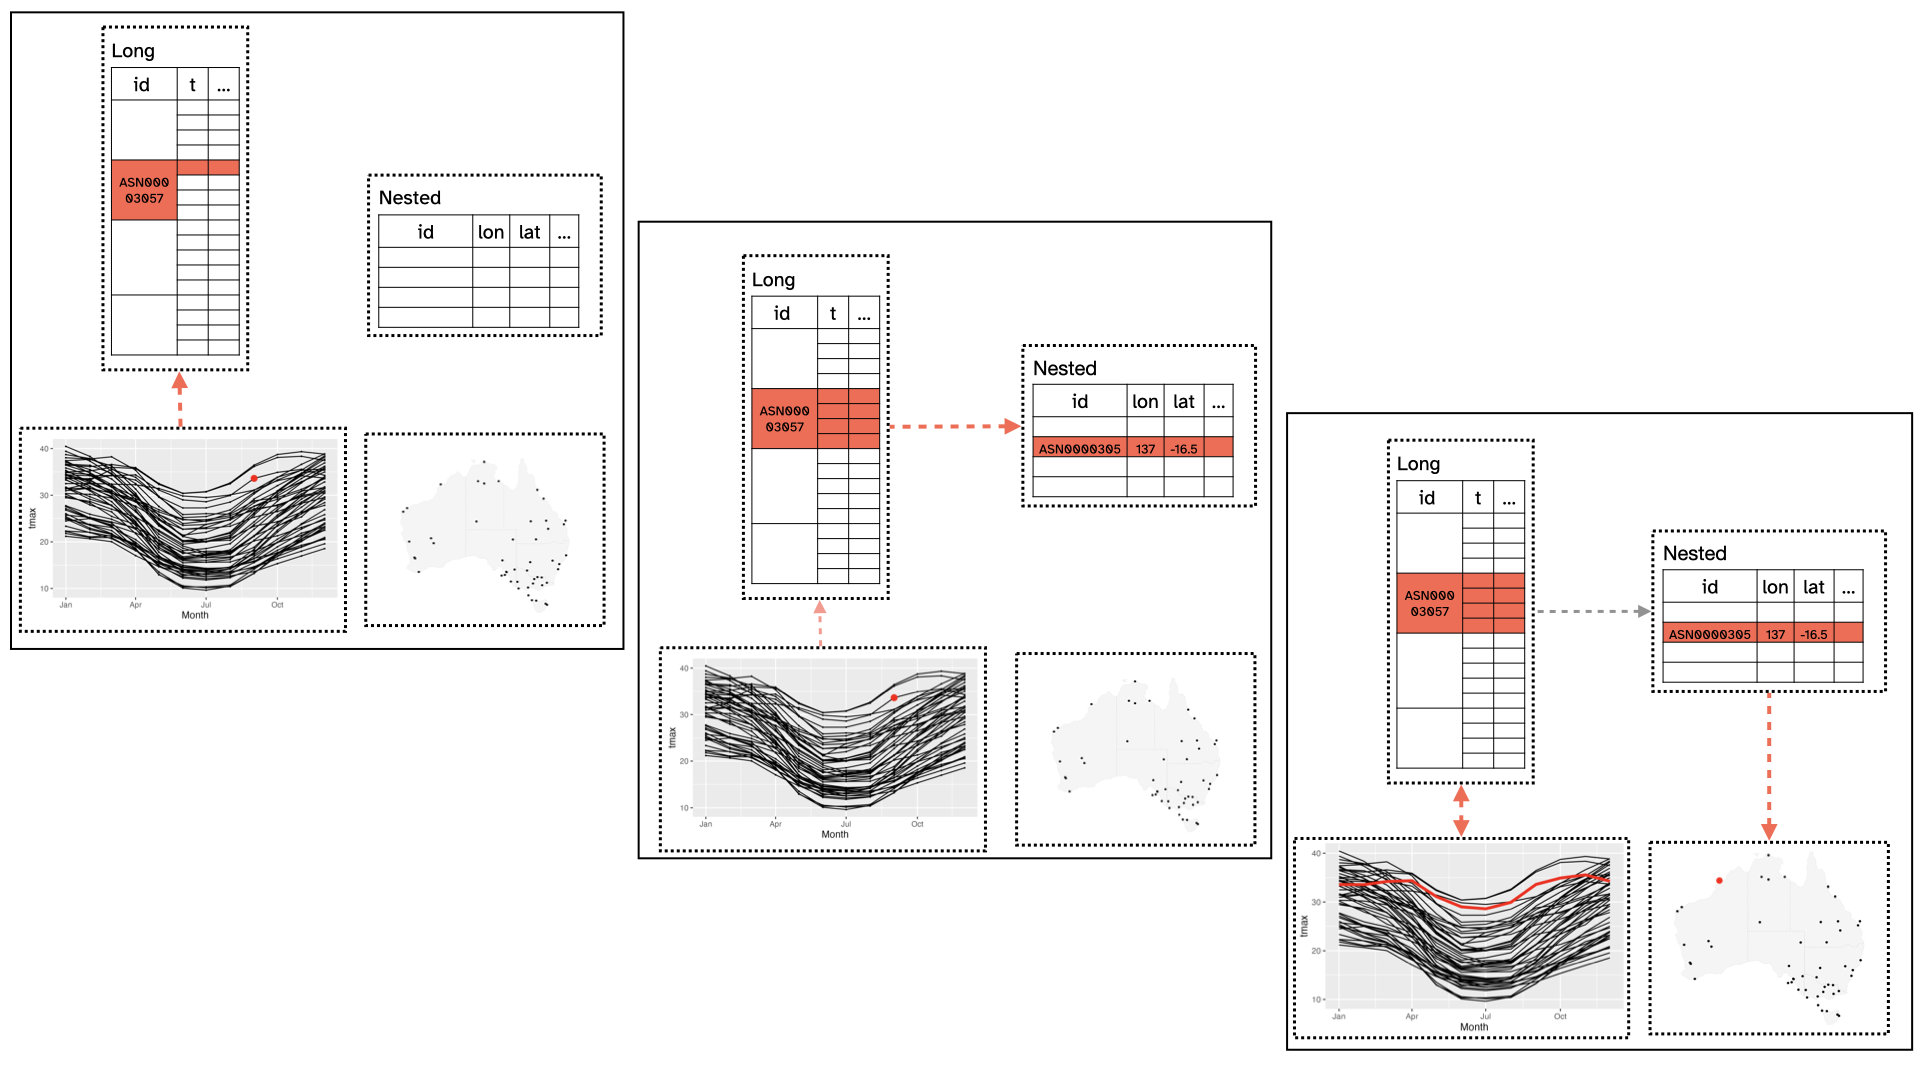
\includegraphics[width=1\linewidth,height=0.4\textheight]{/Users/sherryzhang/Documents/research/paper-cubble/figures/diagram-keynotes/diagram-keynotes.005} 

}

\caption[An illustration of the data model under interactive graphics with cubble]{An illustration of the data model under interactive graphics with cubble. When a point on the time series is selected, the corresponding row in the long cubble will be activated. This will link to all the rows with the same id in the long cubble and the row in the nested cubble with the smae id (middle). Both plots will be updated with the full line selected and the point highlighted on the map (right).}\label{fig:illu-interactive-2}
\end{figure}
\end{CodeChunk}

\newpage

\bibliography{../references.bib}



\end{document}
